% Plain-language review document (explaneat plain-language review), v5.
\documentclass[a4paper,10pt]{article}
\usepackage[margin=1.8cm]{geometry}
\usepackage{amsmath}
\usepackage{amssymb}
\usepackage{booktabs}
\usepackage{tabularx}
\usepackage{graphicx}
\usepackage[table,usenames,dvipsnames]{xcolor}
\usepackage{tikz}
\usetikzlibrary{arrows.meta,fit,backgrounds,positioning,calc}
\usetikzlibrary{shapes.geometric}
\usepackage{longtable}
\usepackage{pdflscape}
\usepackage{float}
\usepackage[font=small,labelfont=bf]{caption}
\usepackage{array}
\usepackage[unicode=true,hidelinks]{hyperref}
\setcounter{tocdepth}{3}
\setcounter{secnumdepth}{3}
% Review markers, copied from dissertation.tex (7 Nov 2026) for standalone builds.
\newif\ifreviewmarks
\reviewmarkstrue
\newcommand{\reviewrule}{\noindent{\color{BrickRed}\rule{\linewidth}{0.8pt}}}
\newenvironment{drafted}[1][]{%
  \ifreviewmarks\par\addvspace{\medskipamount}\reviewrule\par\nopagebreak
  \noindent{\color{BrickRed}\sffamily\footnotesize\textbf{Thesis Draft}\quad #1\hfill review}\par\nopagebreak\smallskip\fi}{%
  \ifreviewmarks\par\smallskip\noindent{\color{BrickRed}\sffamily\footnotesize end of thesis draft}\par\nopagebreak\reviewrule\par\medskip\fi}
\newcommand{\figreview}[1]{\ifreviewmarks\par\smallskip{\color{NavyBlue}\sffamily\footnotesize\textbf{Figure note:} #1}\par\fi}
\begin{document}
\begin{center}{\Large\bfseries Plain-language explanation: heart-s2-c3\par}\vspace{2mm}{\small AI-assisted drafts for review. Nothing here has been verified by a person.\par}\end{center}
\noindent\textbf{How to read this.} Explanations are built up but read down: the summary first, then each part from the whole model down, in plain words, each sentence followed by the claims it rests on (C01, C02, \ldots; every cited claim was computed on the model and checked). Numbers are changes in predicted risk for a typical patient. The technical record (original hypotheses, formulas, evidence tables with the test check, ranges and n) is at the end. The text describes what the model does, not the world; whether it is plausible is for the reviewer to judge.
\par\medskip\noindent\textbf{What changed in v5e (figures).} v5e: every diagram is a numbered figure with a caption (list of figures after the contents) and the text refers to it; the whole-network figure has its own landscape page, scaled to the page, with a short caption and its description in the text; an input used by several parts is drawn under each of them (same input, repeated for readability, dotted outline); and an appendix figure shows the trained network before any explanation (no parts, no splits).
\par\medskip\noindent\textbf{What changed in v5c (tables and diagrams).} v5c: the evidence tables are landscape, compact and shaded by row, with the header repeated on every page (longtable and pdflscape, used in this review PDF only; the thesis preamble has neither). In the diagrams each input is drawn once, in a shared row along the bottom (the explanation's split copies of an input are listed in the technical detail instead), every cluster has one output rectangle with its plain name, the inputs that feed the output directly meet in a drawn 'sum', and a one-line legend explains the edges.
\par\medskip\noindent\textbf{What changed in v5b (diagrams).} v5b uses one grouping everywhere, the annotation hierarchy: the summary's diagram is the same picture as the whole model's section, and a part that is itself a weighted sum (blood pressure with cholesterol) is a part of its own, described as one that adds up, so the text counts three parts throughout; the lint checks every 'N parts' against the hierarchy. A full-structure diagram follows the summary: every node and connection, nested by part, with the inputs that feed the output directly in their own cluster and the unused input columns listed. Each section from the top down adds its own region of that diagram, with stubs for connections from or to other parts; each connection is drawn in exactly one section. The gate's text now says that it lowers the risk for the patients it acts on, and that more vessels and higher cholesterol take that lowering away; its vessel statements are one per group.
\par\medskip\noindent\textbf{What changed in v5 (read down).} v5 reads the explanation down. The summary (one line, a diagram, one paragraph per block) is as in v4, except that the paragraph on what adds up is split into protective items, risk-raising items and rare results, and an input that also feeds a part is quoted with its direct contribution only (the rest is in that part's paragraph). Then the document walks the annotation hierarchy from the whole model down: for each part a plain hypothesis (what it does for the prediction), plain evidence (what was checked and what it showed; for a part made of others, what they are and how they combine), a diagram one level down and where to read on. The original hypotheses, closed forms and evidence tables are in 'Technical detail' at the end. Statements about structure (what a part is made of, a copy of another part, a formula that reproduces it) are now claims of their own, checked on the graph and the data.
\par\medskip\noindent\textbf{v4.} v4 follows the structure of the explanation. The summary opens with one line and a diagram at the same grouping, then gives one paragraph per top-level block of the annotation hierarchy: one for everything that adds up independently (the inputs that feed the model score directly, and parts that are a weighted sum), and one for each part that combines its inputs in another way: what it combines, how, and for whom. 'Parts in detail' follows the hierarchy below that, with a diagram one level down for each part that contains others. The prose no longer says 'clearly', 'slightly', 'consistently' or 'on the training data only': the numbers carry it, and the test check, the ranges and n stay in the evidence tables. Only genuinely small groups are marked, with their n. The lint rejects the confidence words and checks the block structure.
\tableofcontents
\listoffigures
\clearpage
\begin{drafted}[plain-language layer: heart-s2-c3]
\section{heart-s2-c3}
\noindent{\small Genome \texttt{1a5255ec-4f4d-4ff4-916a-1b5c4622ccc9}, explanation \texttt{6565cffd-9c19-4ae2-b635-a2e35f3d485a}. Split: train primary (n=242), test as a check (n=61). Claims: 52, verified 46, not supported 6.\par}
\noindent{\small\textcolor{BrickRed}{AI-assisted draft for review (unverified)}\par}\smallskip
\noindent{\footnotesize Reference (typical) patient: the typical patient: the median training patient for every number and the most common training category for every category (not a real patient). age: 56 years; ca: 0 vessels; chol: 240 mg/dL (6.2 mmol/L); cp: no chest pain (asymptomatic); exang: no chest pain on exercise; fbs: fasting blood sugar of 120 mg/dL or less; oldpeak: 0.8 mm; restecg: a normal resting ECG; sex: male; slope: an upsloping ST segment; thal: a normal thallium scan; thalach: 152 beats per minute; trestbps: 130 mm Hg. Predicted risk of heart disease: 30\%.\par}
\subsection{Summary}
\noindent For a typical patient (a 56-year-old man with no chest pain symptoms and median test results) the model predicts a risk of heart disease of about 30\%; it adds up most of its inputs independently, and three parts that all read chest pain type add to that sum: one acts on 76 of 242 training patients through maximum heart rate, one on 61 through cholesterol, and one barely changes the predictions.\,{\scriptsize\textcolor{NavyBlue}{[C29, C34, C40, C50]}} Figure~\ref{fig:hearts2c3:summary} shows the model at this level: one box per paragraph below.
\par\medskip\noindent\fbox{\begin{minipage}{0.96\linewidth}\small\textbf{How to read the diagrams.} Edge colour is the sign of that one connection: blue positive, red negative; thicker is a larger weight. The outline and arrow on an input (and on a part's output box) is its overall effect on the final prediction, read from the verified claims: orange and up arrow raises it, teal and down arrow lowers it, grey and double arrow depends (it goes both ways, or differs between levels). A negative connection into a part that itself raises the prediction means that input lowers the prediction; through a hinge the overall effect can only be read from the claims, not from the edges. Up arrow means towards heart disease; down arrow, away from it. A double outline marks an input (or a part's output) that acts at a fixed rate everywhere: it adds the same amount to the score per unit, so it is explained by its rate alone (see 'Linear factors'); a dashed double outline, at a fixed rate on the observed data. The normal outline is an input whose effect switches on and off somewhere. For example, non-anginal pain has a negative connection into 'ST depression gate with little effect', a part that lowers the predicted risk of heart disease, so non-anginal pain raises it.\end{minipage}}\par\medskip
\begin{figure}[H]\centering
\resizebox{!}{\ifdim\height>0.5\textheight 0.5\textheight\else\height\fi}{%
\resizebox{\ifdim\width>\linewidth\linewidth\else\width\fi}{!}{%
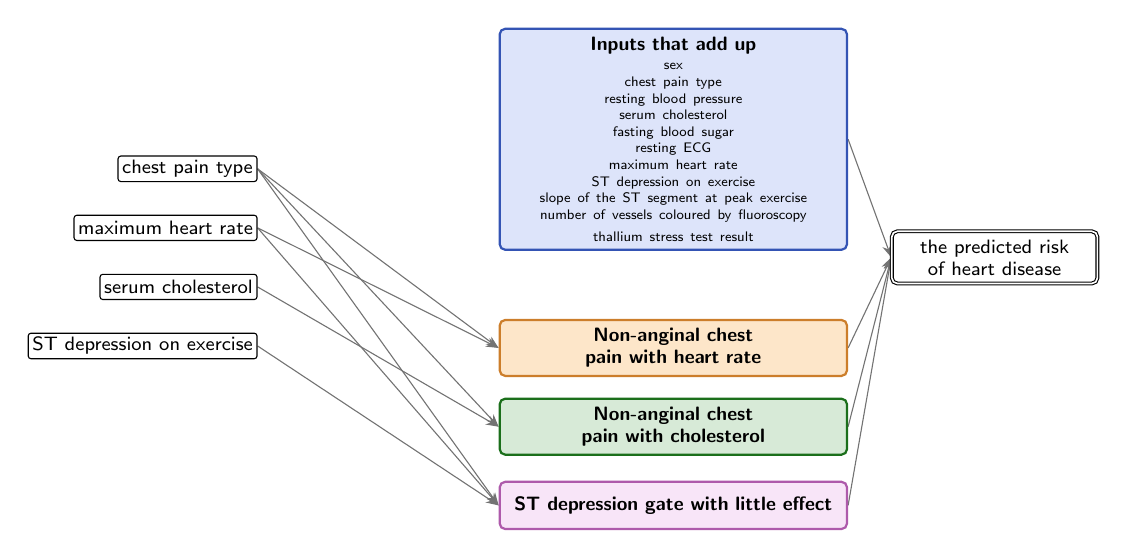
\begin{tikzpicture}[
  font=\sffamily\scriptsize, >={Stealth[length=1.6mm]},
  inp/.style={draw, rounded corners=1pt, fill=white, inner sep=1.5pt, minimum height=3.2mm, anchor=east},
  abox/.style={draw, thick, rounded corners=2pt, align=center, inner sep=3pt, minimum height=6mm, text width=42mm},
  outp/.style={draw, double, rounded corners=2pt, fill=white, align=center, inner sep=3pt, text width=24mm},
  agg/.style={draw=black!55},
]
\node[inp] (i0) at (0,1.125) {chest pain type};
\node[inp] (i1) at (0,0.375) {maximum heart rate};
\node[inp] (i2) at (0,-0.375) {serum cholesterol};
\node[inp] (i3) at (0,-1.125) {ST depression on exercise};
\node[abox, fill=RoyalBlue!18, draw=RoyalBlue!80!black] (b0) at (5.28,1.5) {\textbf{Inputs that add up}\\[1pt]{\tiny sex\\ chest pain type\\ resting blood pressure\\ serum cholesterol\\ fasting blood sugar\\ resting ECG\\ maximum heart rate\\ ST depression on exercise\\ slope of the ST segment at peak exercise\\ number of vessels coloured by fluoroscopy\\ thallium stress test result}};
\node[abox, fill=BurntOrange!18, draw=BurntOrange!80!black] (b1) at (5.28,-1.15) {\textbf{Non-anginal chest pain with heart rate}};
\node[abox, fill=ForestGreen!18, draw=ForestGreen!80!black] (b2) at (5.28,-2.15) {\textbf{Non-anginal chest pain with cholesterol}};
\node[abox, fill=Orchid!18, draw=Orchid!80!black] (b3) at (5.28,-3.15) {\textbf{ST depression gate with little effect}};
\node[outp] (out) at (9.36,0) {the predicted risk of heart disease};
\begin{scope}[on background layer]
\draw[->, agg] (b0.east) -- (out.west);
\draw[->, agg, thin] (i0.east) -- (b1.west);
\draw[->, agg, thin] (i1.east) -- (b1.west);
\draw[->, agg] (b1.east) -- (out.west);
\draw[->, agg, thin] (i0.east) -- (b2.west);
\draw[->, agg, thin] (i2.east) -- (b2.west);
\draw[->, agg] (b2.east) -- (out.west);
\draw[->, agg, thin] (i0.east) -- (b3.west);
\draw[->, agg, thin] (i1.east) -- (b3.west);
\draw[->, agg, thin] (i3.east) -- (b3.west);
\draw[->, agg] (b3.east) -- (out.west);
\end{scope}
\end{tikzpicture}}}%
\caption{The model at the level of the summary: one box per part.}
\label{fig:hearts2c3:summary}
\end{figure}
\paragraph{Inputs that add up.} \par\noindent\textit{Lowering the risk.}  These add up independently, and these lower the risk: through this sum alone, compared with no chest pain symptoms, typical angina takes a typical patient's predicted risk from about 30\% to about 2\%, non-anginal chest pain to about 7\% and atypical angina to about 13\% (chest pain type also acts through the parts below); being a woman lowers it to about 4\% and fasting blood sugar above 120 mg/dL to about 19\%; and through this sum alone a higher maximum heart rate lowers it steadily, from about 36\% at 118 to about 27\% at 175 beats per minute (it also acts through the parts below).\,{\scriptsize\textcolor{NavyBlue}{[C05, C14, C16, C10, C18, C19]}} \par\noindent\textit{Raising the risk.}  Each extra vessel coloured by fluoroscopy adds about the same, from about 30\% at 0 to about 96\% at 2 vessels, flattening out near the top because the predicted risk cannot go much higher; a flat rather than upsloping ST segment raises it to about 80\%, higher resting blood pressure raises it steadily from about 20\% at 110 mm Hg to about 46\% at 155 mm Hg, and a reversible defect on the thallium scan raises it to about 55\%.\,{\scriptsize\textcolor{NavyBlue}{[C01, C02, C11, C12]}} Through this sum alone, more ST depression on exercise raises it steadily from about 23\% at 0 mm to about 53\% at 2.8 mm, and higher cholesterol raises it steadily from about 21\% at 193 mg/dL to about 48\% at 308 mg/dL; both also act through the parts below.\,{\scriptsize\textcolor{NavyBlue}{[C03, C07]}} \par\noindent\textit{Rare results.}  Some rarer results also count (the model has little data on this, n = 15 to 17): a downsloping ST segment raises the risk to about 54\% and a fixed defect on the thallium scan lowers it to about 12\%, while signs of left ventricular hypertrophy on the resting ECG raise it from about 30\% to about 33\%.\,{\scriptsize\textcolor{NavyBlue}{[C13, C15, C21]}}
\paragraph{Non-anginal chest pain with heart rate.} This part reads chest pain type and maximum heart rate, and acts on 76 of 242 training patients, mostly patients with non-anginal chest pain, 15 of whom had heart disease; for the typical patient it acts on, the predicted risk is about 5\% without it and about 2\% with it.\,{\scriptsize\textcolor{NavyBlue}{[C34]}} Through it, non-anginal chest pain rather than any other chest pain type takes a typical patient's predicted risk from about 30\% to about 17\%.\,{\scriptsize\textcolor{NavyBlue}{[C30]}} Across the whole model, a higher maximum heart rate lowers the risk slowly at first, then faster, and more with non-anginal chest pain: from about 7\% at 118 to about 2\% at 175 beats per minute then, flattening out near the bottom because the predicted risk cannot go much lower, against about 36\% to about 27\% for other chest pain types.\,{\scriptsize\textcolor{NavyBlue}{[C32]}}
\paragraph{Non-anginal chest pain with cholesterol.} This part reads chest pain type and cholesterol, and acts on 61 of 242 training patients, all of them with non-anginal chest pain, 13 of whom had heart disease; for the typical patient it acts on, the predicted risk is about 3\% without it and about 2\% with it.\,{\scriptsize\textcolor{NavyBlue}{[C40]}} Through it, for patients with non-anginal chest pain, higher cholesterol raises the predicted risk steadily up to about 282 mg/dL, where the part switches off, then no further: for the typical patient it acts on, from about 2\% at 193 mg/dL to about 3\% at 308 mg/dL.\,{\scriptsize\textcolor{NavyBlue}{[C37, C39]}} Across the whole model, higher cholesterol raises the risk in an uneven way from about 2\% to about 7\% with non-anginal chest pain, against about 21\% to about 48\% for other chest pain types.\,{\scriptsize\textcolor{NavyBlue}{[C38]}}
\paragraph{ST depression gate with little effect.} This part reads chest pain type, maximum heart rate and ST depression on exercise, and barely changes the predictions (by at most 0.5 percentage points).\,{\scriptsize\textcolor{NavyBlue}{[C50]}} It switches on when ST depression on exercise minus about 0.019 $\times$ the maximum heart rate exceeds about -1.71, which never happens with non-anginal chest pain; 73 of 242 training patients are on, and 79\% of them had heart disease, against 29\% of the others.\,{\scriptsize\textcolor{NavyBlue}{[C52]}}
\paragraph{The whole network.} Figure~\ref{fig:hearts2c3:overview} (next page, landscape) draws every unit and connection of the explained model, nested by part: shaded clusters are the parts of the model and darker boxes the parts inside them; circles are hidden units (h1, h2, \ldots); each cluster's rectangle is its output, and a dashed `sum' stands for an addition the next unit does (drawn, not a unit of the model); the hexagon is the model's output. An input used by several parts is drawn under each of them (same label, dotted outline, the first copy marked with the number of copies): it is the same input, repeated for readability. Not used by the model (input columns with no connection): age, sugar 120 or less, normal ECG, ST-T abnormal ECG, no exercise pain, exercise pain, downsloping ST, normal thallium, thallium code 4.
\begin{landscape}
\begin{figure}[p]\centering
\resizebox{\linewidth}{!}{%
\definecolor{netup}{HTML}{D95F02}\definecolor{netdown}{HTML}{1B9E77}\definecolor{netmixed}{HTML}{7F7F7F}%
\begin{tikzpicture}[
  font=\sffamily\scriptsize, >={Stealth[length=1.4mm]},
  inp/.style={draw, circle, fill=white, minimum size=3.2mm, inner sep=0pt},
  hid/.style={draw, circle, fill=white, minimum size=5.2mm, inner sep=0.5pt, font=\sffamily\tiny},
  exitbox/.style={draw, thick, rectangle, fill=white, align=center, text width=17mm, minimum height=5mm, inner sep=1.5pt, font=\sffamily\tiny},
  sumbox/.style={draw, thick, dashed, rectangle, fill=white, align=center, text width=17mm, minimum height=5mm, inner sep=1.5pt, font=\sffamily\tiny},
  outp/.style={draw, thick, regular polygon, regular polygon sides=6, fill=white, minimum size=10mm, inner sep=0pt, font=\sffamily\tiny, align=center},
  stub/.style={draw, dashed, rounded corners=2pt, fill=white, align=center, inner sep=2pt, font=\sffamily\tiny, text width=15mm},
  inlab/.style={font=\sffamily\tiny, align=center, text width=15mm, inner sep=1pt, fill=white, fill opacity=0.8, text opacity=1},
  wpos/.style={draw=NavyBlue}, wneg/.style={draw=BrickRed}, wagg/.style={draw=black!45, line width=1.2pt},
  wmix/.style={draw=Plum},
]
\node[outp] (n0) at (19.06,3.45) {heart disease};
\node[exitbox] (n2472) at (17.04,1.9) {Non-anginal chest pain with heart rate $\downarrow$};
\node[exitbox] (n2596) at (35.42,1.9) {ST depression gate with little effect $\downarrow$};
\node[exitbox] (n2863) at (26.28,1.9) {Non-anginal chest pain with cholesterol $\downarrow$};
\node[sumbox] (nxxsumxx) at (5.85,1.9) {sum: Inputs that add up};
\node[inp, draw=netdown, very thick] (ninxxsexx0xxadditive) at (3.6,-1.05) {};
\path (ninxxsexx0xxadditive.south) node[inlab, anchor=north] (labninxxsexx0xxadditive) {female $\downarrow$};
\node[inp, draw=netup, very thick] (ninxxsexx1xxadditive) at (5.4,-1.05) {};
\path (ninxxsexx1xxadditive.south) node[inlab, anchor=north] (labninxxsexx1xxadditive) {male $\uparrow$};
\node[inp, draw=netdown, very thick] (ninxxcpx1xxadditive) at (9.0,-1.05) {};
\path (ninxxcpx1xxadditive.south) node[inlab, anchor=north] (labninxxcpx1xxadditive) {typical angina $\downarrow$};
\node[inp, draw=netdown, very thick] (ninxxcpx2xxadditive) at (1.8,-1.05) {};
\path (ninxxcpx2xxadditive.south) node[inlab, anchor=north] (labninxxcpx2xxadditive) {atypical angina $\downarrow$};
\node[inp, draw=netup, very thick] (ninxxcpx4xxadditive) at (6.3,-2.1) {};
\path (ninxxcpx4xxadditive.south) node[inlab, anchor=north] (labninxxcpx4xxadditive) {no chest pain $\uparrow$};
\node[inp, draw=netup, very thick] (ninxxtrestbpsxxadditive) at (2.7,0.0) {};
\path (ninxxtrestbpsxxadditive.south) node[inlab, anchor=north] (labninxxtrestbpsxxadditive) {blood pressure $\uparrow$};
\node[inp, draw=netdown, very thick] (ninxxfbsx1xxadditive) at (8.1,0.0) {};
\path (ninxxfbsx1xxadditive.south) node[inlab, anchor=north] (labninxxfbsx1xxadditive) {sugar above 120 $\downarrow$};
\node[inp, draw=netup, very thick] (ninxxrestecgx2xxadditive) at (0.9,0.0) {};
\path (ninxxrestecgx2xxadditive.south) node[inlab, anchor=north] (labninxxrestecgx2xxadditive) {LVH on ECG $\uparrow$};
\node[inp, draw=netdown, very thick] (ninxxslopex1xxadditive) at (9.9,0.0) {};
\path (ninxxslopex1xxadditive.south) node[inlab, anchor=north] (labninxxslopex1xxadditive) {upsloping ST $\downarrow$};
\node[inp, draw=netup, very thick] (ninxxslopex2xxadditive) at (4.5,-2.1) {};
\path (ninxxslopex2xxadditive.south) node[inlab, anchor=north] (labninxxslopex2xxadditive) {flat ST $\uparrow$};
\node[inp, draw=netup, very thick] (ninxxcaxxadditive) at (10.8,-1.05) {};
\path (ninxxcaxxadditive.south) node[inlab, anchor=north] (labninxxcaxxadditive) {vessels $\uparrow$};
\node[inp, draw=netdown, very thick] (ninxxthalx6xxadditive) at (4.5,0.0) {};
\path (ninxxthalx6xxadditive.south) node[inlab, anchor=north] (labninxxthalx6xxadditive) {fixed defect $\downarrow$};
\node[inp, draw=netup, very thick] (ninxxthalx7xxadditive) at (7.2,-1.05) {};
\path (ninxxthalx7xxadditive.south) node[inlab, anchor=north] (labninxxthalx7xxadditive) {reversible defect $\uparrow$};
\node[inp, densely dotted, thick, draw=netdown, very thick] (ninxxcpx3xxannx30) at (17.94,0.0) {};
\path (ninxxcpx3xxannx30.south) node[inlab, anchor=north] (labninxxcpx3xxannx30) {non-anginal pain ($\times$3) $\downarrow$};
\node[inp, densely dotted, thick, draw=netup, very thick] (ninxxcpx3xxannx31) at (37.22,0.0) {};
\path (ninxxcpx3xxannx31.south) node[inlab, anchor=north] (labninxxcpx3xxannx31) {non-anginal pain $\uparrow$};
\node[inp, densely dotted, thick, draw=netdown, very thick] (ninxxcpx3xxannx32) at (27.18,0.0) {};
\path (ninxxcpx3xxannx32.south) node[inlab, anchor=north] (labninxxcpx3xxannx32) {non-anginal pain $\downarrow$};
\node[inp, densely dotted, thick, draw=netdown, very thick] (ninxxthalachxxadditive) at (6.3,0.0) {};
\path (ninxxthalachxxadditive.south) node[inlab, anchor=north] (labninxxthalachxxadditive) {max heart rate ($\times$3) $\downarrow$};
\node[inp, densely dotted, thick, draw=netdown, very thick] (ninxxthalachxxannx30) at (16.14,0.0) {};
\path (ninxxthalachxxannx30.south) node[inlab, anchor=north] (labninxxthalachxxannx30) {max heart rate $\downarrow$};
\node[inp, densely dotted, thick, draw=netup, very thick] (ninxxthalachxxannx31) at (35.42,0.0) {};
\path (ninxxthalachxxannx31.south) node[inlab, anchor=north] (labninxxthalachxxannx31) {max heart rate $\uparrow$};
\node[inp, densely dotted, thick, draw=netup, very thick] (ninxxoldpeakxxadditive) at (0.9,-2.1) {};
\path (ninxxoldpeakxxadditive.south) node[inlab, anchor=north] (labninxxoldpeakxxadditive) {ST depression ($\times$2) $\uparrow$};
\node[inp, densely dotted, thick, draw=netdown, very thick] (ninxxoldpeakxxannx31) at (33.62,0.0) {};
\path (ninxxoldpeakxxannx31.south) node[inlab, anchor=north] (labninxxoldpeakxxannx31) {ST depression $\downarrow$};
\node[inp, densely dotted, thick, draw=netup, very thick] (ninxxcholxxadditive) at (2.7,-2.1) {};
\path (ninxxcholxxadditive.south) node[inlab, anchor=north] (labninxxcholxxadditive) {cholesterol ($\times$2) $\uparrow$};
\node[inp, densely dotted, thick, draw=netup, very thick] (ninxxcholxxannx32) at (25.38,0.0) {};
\path (ninxxcholxxannx32.south) node[inlab, anchor=north] (labninxxcholxxannx32) {cholesterol $\uparrow$};
\begin{scope}[on background layer]
\node[fit=(nxxsumxx) , inner sep=8pt, rounded corners=5pt, fill=RoyalBlue!10, draw=RoyalBlue!45] (clu0) {};
\node[fit=(n2472) , inner sep=8pt, rounded corners=5pt, fill=BurntOrange!10, draw=BurntOrange!45] (clu1) {};
\node[fit=(n2863) , inner sep=8pt, rounded corners=5pt, fill=ForestGreen!10, draw=ForestGreen!45] (clu2) {};
\node[fit=(n2596) , inner sep=8pt, rounded corners=5pt, fill=Orchid!10, draw=Orchid!45] (clu3) {};
\draw[->, wneg, line width=0.52pt] (ninxxsexx0xxadditive) -- (nxxsumxx);
\draw[->, wpos, line width=0.37pt] (ninxxsexx1xxadditive) -- (nxxsumxx);
\draw[->, wneg, line width=0.39pt] (ninxxcpx1xxadditive) -- (nxxsumxx);
\draw[->, wpos, line width=0.35pt] (ninxxcpx2xxadditive) -- (nxxsumxx);
\draw[->, wpos, line width=0.55pt] (ninxxcpx4xxadditive) -- (nxxsumxx);
\draw[->, wpos, line width=0.42pt] (ninxxtrestbpsxxadditive) -- (nxxsumxx);
\draw[->, wneg, line width=0.32pt] (ninxxfbsx1xxadditive) -- (nxxsumxx);
\draw[->, wpos, line width=0.27pt] (ninxxrestecgx2xxadditive) -- (nxxsumxx);
\draw[->, wneg, line width=0.42pt] (ninxxslopex1xxadditive) -- (nxxsumxx);
\draw[->, wpos, line width=0.46pt] (ninxxslopex2xxadditive) -- (nxxsumxx);
\draw[->, wpos, line width=0.87pt] (ninxxcaxxadditive) -- (nxxsumxx);
\draw[->, wneg, line width=0.35pt] (ninxxthalx6xxadditive) -- (nxxsumxx);
\draw[->, wpos, line width=0.42pt] (ninxxthalx7xxadditive) -- (nxxsumxx);
\draw[->, wneg, line width=0.43pt] (n2472) -- (n0);
\draw[->, wneg, line width=0.26pt] (n2596) -- (n0);
\draw[->, wneg, line width=0.33pt] (n2863) -- (n0);
\draw[->, wpos, line width=0.63pt] (ninxxcpx3xxannx30) -- (n2472);
\draw[->, wneg, line width=0.59pt] (ninxxcpx3xxannx31) -- (n2596);
\draw[->, wpos, line width=0.59pt] (ninxxcpx3xxannx32) -- (n2863);
\draw[->, wneg, line width=0.31pt] (ninxxthalachxxadditive) -- (nxxsumxx);
\draw[->, wpos, line width=0.49pt] (ninxxthalachxxannx30) -- (n2472);
\draw[->, wneg, line width=0.33pt] (ninxxthalachxxannx31) -- (n2596);
\draw[->, wpos, line width=0.45pt] (ninxxoldpeakxxadditive) -- (nxxsumxx);
\draw[->, wpos, line width=0.49pt] (ninxxoldpeakxxannx31) -- (n2596);
\draw[->, wpos, line width=0.44pt] (ninxxcholxxadditive) -- (nxxsumxx);
\draw[->, wneg, line width=0.38pt] (ninxxcholxxannx32) -- (n2863);
\draw[->, wagg] (nxxsumxx) -- (n0);
\end{scope}
\node[font=\sffamily\scriptsize\bfseries, text=RoyalBlue!55!black, anchor=south west, inner sep=1pt, fill=white, fill opacity=0.85, text opacity=1] at (clu0.north west) {Inputs that add up};
\node[font=\sffamily\scriptsize\bfseries, text=BurntOrange!55!black, anchor=south west, inner sep=1pt, fill=white, fill opacity=0.85, text opacity=1] at (clu1.north west) {Non-anginal chest pain with heart rate};
\node[font=\sffamily\scriptsize\bfseries, text=ForestGreen!55!black, anchor=south west, inner sep=1pt, fill=white, fill opacity=0.85, text opacity=1] at (clu2.north west) {Non-anginal chest pain with cholesterol};
\node[font=\sffamily\scriptsize\bfseries, text=Orchid!55!black, anchor=south west, inner sep=1pt, fill=white, fill opacity=0.85, text opacity=1] at (clu3.north west) {ST depression gate with little effect};
\end{tikzpicture}}%
\caption{Every unit and connection of the explained model, nested by part. Blue: positive weight (raises the score); red: negative weight (lowers it); thicker: larger weight. Orange outline and up arrow: raises the final prediction; teal and down arrow: lowers it; grey and double arrow: depends.}
\label{fig:hearts2c3:overview}
\end{figure}
\end{landscape}
\paragraph{Worth checking against what is known.} Worth checking: going from 0 to 2 vessels coloured moves a typical patient's predicted risk from about 30\% to about 96\%.\,{\scriptsize\textcolor{NavyBlue}{[C01]}} Worth checking: patients with typical angina get the lowest predicted risk of all chest pain types (about 2\%), below non-anginal chest pain (about 3\%), atypical angina (about 13\%) and no chest pain symptoms (about 30\%).\,{\scriptsize\textcolor{NavyBlue}{[C06, C09, C17]}} Worth checking: the model treats fasting blood sugar above 120 mg/dL as lowering the risk of heart disease (for a typical patient from about 30\% to about 19\%).\,{\scriptsize\textcolor{NavyBlue}{[C18]}} Worth checking: the model treats a fixed defect on the thallium scan as lowering the risk (for a typical patient from about 30\% to about 12\%), from only 15 training patients.\,{\scriptsize\textcolor{NavyBlue}{[C15]}} Worth checking: the model ignores age.\,{\scriptsize\textcolor{NavyBlue}{[C27]}} Worth checking: with non-anginal chest pain, one part lowers the predicted risk for cholesterol below about 282 mg/dL, so cholesterol moves the risk from about 2\% to about 7\% for these patients, against about 21\% to about 48\% for others.\,{\scriptsize\textcolor{NavyBlue}{[C38, C39]}}
\subsection{The model, read from the top down}
\noindent{\small Each part of the explanation in turn, from the whole model down to the smallest parts: what it does for the prediction (hypothesis), what was checked (evidence), a diagram one level down, and where to read on. The technical record of each part is in ``Technical detail'' at the end.\par}
\subsubsection{The whole model}\label{rd:ann33}
\noindent{\small Figure~\ref{fig:hearts2c3:parts-ann33} shows what feeds this part; Figure~\ref{fig:hearts2c3:units-ann33} its units and every connection into them (dashed boxes: connections from or to other parts, drawn in their own sections).\par}
\begin{figure}[H]\centering
\resizebox{!}{\ifdim\height>0.5\textheight 0.5\textheight\else\height\fi}{%
\resizebox{\ifdim\width>\linewidth\linewidth\else\width\fi}{!}{%
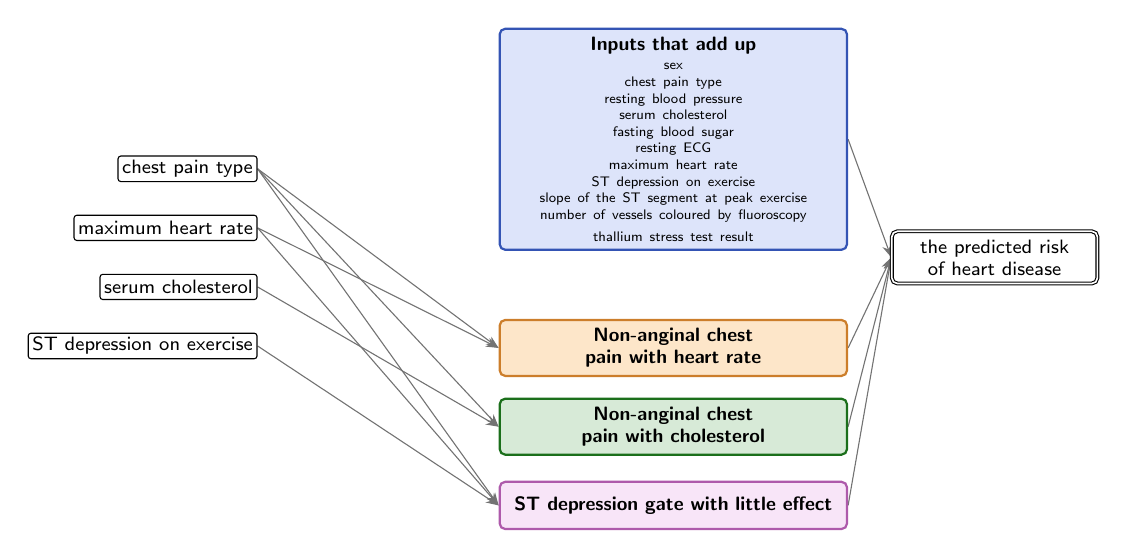
\begin{tikzpicture}[
  font=\sffamily\scriptsize, >={Stealth[length=1.6mm]},
  inp/.style={draw, rounded corners=1pt, fill=white, inner sep=1.5pt, minimum height=3.2mm, anchor=east},
  abox/.style={draw, thick, rounded corners=2pt, align=center, inner sep=3pt, minimum height=6mm, text width=42mm},
  outp/.style={draw, double, rounded corners=2pt, fill=white, align=center, inner sep=3pt, text width=24mm},
  agg/.style={draw=black!55},
]
\node[inp] (i0) at (0,1.125) {chest pain type};
\node[inp] (i1) at (0,0.375) {maximum heart rate};
\node[inp] (i2) at (0,-0.375) {serum cholesterol};
\node[inp] (i3) at (0,-1.125) {ST depression on exercise};
\node[abox, fill=RoyalBlue!18, draw=RoyalBlue!80!black] (b0) at (5.28,1.5) {\textbf{Inputs that add up}\\[1pt]{\tiny sex\\ chest pain type\\ resting blood pressure\\ serum cholesterol\\ fasting blood sugar\\ resting ECG\\ maximum heart rate\\ ST depression on exercise\\ slope of the ST segment at peak exercise\\ number of vessels coloured by fluoroscopy\\ thallium stress test result}};
\node[abox, fill=BurntOrange!18, draw=BurntOrange!80!black] (b1) at (5.28,-1.15) {\textbf{Non-anginal chest pain with heart rate}};
\node[abox, fill=ForestGreen!18, draw=ForestGreen!80!black] (b2) at (5.28,-2.15) {\textbf{Non-anginal chest pain with cholesterol}};
\node[abox, fill=Orchid!18, draw=Orchid!80!black] (b3) at (5.28,-3.15) {\textbf{ST depression gate with little effect}};
\node[outp] (out) at (9.36,0) {the predicted risk of heart disease};
\begin{scope}[on background layer]
\draw[->, agg] (b0.east) -- (out.west);
\draw[->, agg, thin] (i0.east) -- (b1.west);
\draw[->, agg, thin] (i1.east) -- (b1.west);
\draw[->, agg] (b1.east) -- (out.west);
\draw[->, agg, thin] (i0.east) -- (b2.west);
\draw[->, agg, thin] (i2.east) -- (b2.west);
\draw[->, agg] (b2.east) -- (out.west);
\draw[->, agg, thin] (i0.east) -- (b3.west);
\draw[->, agg, thin] (i1.east) -- (b3.west);
\draw[->, agg, thin] (i3.east) -- (b3.west);
\draw[->, agg] (b3.east) -- (out.west);
\end{scope}
\end{tikzpicture}}}%
\caption{The whole model: what feeds it, one level down.}
\label{fig:hearts2c3:parts-ann33}
\end{figure}
\begin{figure}[H]\centering
\resizebox{\ifdim\width>\linewidth\linewidth\else\width\fi}{!}{%
\definecolor{netup}{HTML}{D95F02}\definecolor{netdown}{HTML}{1B9E77}\definecolor{netmixed}{HTML}{7F7F7F}%
\begin{tikzpicture}[
  font=\sffamily\scriptsize, >={Stealth[length=1.4mm]},
  inp/.style={draw, circle, fill=white, minimum size=3.2mm, inner sep=0pt},
  hid/.style={draw, circle, fill=white, minimum size=5.2mm, inner sep=0.5pt, font=\sffamily\tiny},
  exitbox/.style={draw, thick, rectangle, fill=white, align=center, text width=17mm, minimum height=5mm, inner sep=1.5pt, font=\sffamily\tiny},
  sumbox/.style={draw, thick, dashed, rectangle, fill=white, align=center, text width=17mm, minimum height=5mm, inner sep=1.5pt, font=\sffamily\tiny},
  outp/.style={draw, thick, regular polygon, regular polygon sides=6, fill=white, minimum size=10mm, inner sep=0pt, font=\sffamily\tiny, align=center},
  stub/.style={draw, dashed, rounded corners=2pt, fill=white, align=center, inner sep=2pt, font=\sffamily\tiny, text width=15mm},
  inlab/.style={font=\sffamily\tiny, align=center, text width=15mm, inner sep=1pt, fill=white, fill opacity=0.8, text opacity=1},
  wpos/.style={draw=NavyBlue}, wneg/.style={draw=BrickRed}, wagg/.style={draw=black!45, line width=1.2pt},
  wmix/.style={draw=Plum},
]
\node[outp] (n0) at (9.32,3.45) {heart disease};
\node[inp, draw=netdown, very thick] (ninxxsexx0) at (3.6,-1.05) {};
\path (ninxxsexx0.south) node[inlab, anchor=north] (labninxxsexx0) {female $\downarrow$};
\node[sumbox] (nxxsumxx) at (5.85,1.9) {sum: Inputs that add up};
\node[inp, draw=netup, very thick] (ninxxsexx1) at (5.4,-1.05) {};
\path (ninxxsexx1.south) node[inlab, anchor=north] (labninxxsexx1) {male $\uparrow$};
\node[inp, draw=netdown, very thick] (ninxxcpx1) at (9.0,-1.05) {};
\path (ninxxcpx1.south) node[inlab, anchor=north] (labninxxcpx1) {typical angina $\downarrow$};
\node[inp, draw=netdown, very thick] (ninxxcpx2) at (1.8,-1.05) {};
\path (ninxxcpx2.south) node[inlab, anchor=north] (labninxxcpx2) {atypical angina $\downarrow$};
\node[inp, draw=netup, very thick] (ninxxcpx4) at (6.3,-2.1) {};
\path (ninxxcpx4.south) node[inlab, anchor=north] (labninxxcpx4) {no chest pain $\uparrow$};
\node[inp, draw=netup, very thick] (ninxxtrestbps) at (2.7,0.0) {};
\path (ninxxtrestbps.south) node[inlab, anchor=north] (labninxxtrestbps) {blood pressure $\uparrow$};
\node[inp, draw=netdown, very thick] (ninxxfbsx1) at (8.1,0.0) {};
\path (ninxxfbsx1.south) node[inlab, anchor=north] (labninxxfbsx1) {sugar above 120 $\downarrow$};
\node[inp, draw=netup, very thick] (ninxxrestecgx2) at (0.9,0.0) {};
\path (ninxxrestecgx2.south) node[inlab, anchor=north] (labninxxrestecgx2) {LVH on ECG $\uparrow$};
\node[inp, draw=netdown, very thick] (ninxxslopex1) at (9.9,0.0) {};
\path (ninxxslopex1.south) node[inlab, anchor=north] (labninxxslopex1) {upsloping ST $\downarrow$};
\node[inp, draw=netup, very thick] (ninxxslopex2) at (4.5,-2.1) {};
\path (ninxxslopex2.south) node[inlab, anchor=north] (labninxxslopex2) {flat ST $\uparrow$};
\node[inp, draw=netup, very thick] (ninxxca) at (10.8,-1.05) {};
\path (ninxxca.south) node[inlab, anchor=north] (labninxxca) {vessels $\uparrow$};
\node[inp, draw=netdown, very thick] (ninxxthalx6) at (4.5,0.0) {};
\path (ninxxthalx6.south) node[inlab, anchor=north] (labninxxthalx6) {fixed defect $\downarrow$};
\node[inp, draw=netup, very thick] (ninxxthalx7) at (7.2,-1.05) {};
\path (ninxxthalx7.south) node[inlab, anchor=north] (labninxxthalx7) {reversible defect $\uparrow$};
\node[stub] (nfromxxNonmanginalxchestxpainxwithxheartxrate) at (15.94,0.0) {from Non-anginal chest pain with heart rate};
\node[stub] (nfromxxSTxdepressionxgatexwithxlittlexeffect) at (17.74,0.0) {from ST depression gate with little effect};
\node[stub] (nfromxxNonmanginalxchestxpainxwithxcholesterol) at (14.14,0.0) {from Non-anginal chest pain with cholesterol};
\node[inp, draw=netdown, very thick] (ninxxthalach) at (6.3,0.0) {};
\path (ninxxthalach.south) node[inlab, anchor=north] (labninxxthalach) {max heart rate $\downarrow$};
\node[inp, draw=netup, very thick] (ninxxoldpeak) at (0.9,-2.1) {};
\path (ninxxoldpeak.south) node[inlab, anchor=north] (labninxxoldpeak) {ST depression $\uparrow$};
\node[inp, draw=netup, very thick] (ninxxchol) at (2.7,-2.1) {};
\path (ninxxchol.south) node[inlab, anchor=north] (labninxxchol) {cholesterol $\uparrow$};
\begin{scope}[on background layer]
\node[fit=(nxxsumxx) , inner sep=8pt, rounded corners=5pt, fill=RoyalBlue!10, draw=RoyalBlue!45] (clu0) {};
\draw[->, wneg, line width=0.52pt] (ninxxsexx0) -- (nxxsumxx);
\draw[->, wpos, line width=0.37pt] (ninxxsexx1) -- (nxxsumxx);
\draw[->, wneg, line width=0.39pt] (ninxxcpx1) -- (nxxsumxx);
\draw[->, wpos, line width=0.35pt] (ninxxcpx2) -- (nxxsumxx);
\draw[->, wpos, line width=0.55pt] (ninxxcpx4) -- (nxxsumxx);
\draw[->, wpos, line width=0.42pt] (ninxxtrestbps) -- (nxxsumxx);
\draw[->, wneg, line width=0.32pt] (ninxxfbsx1) -- (nxxsumxx);
\draw[->, wpos, line width=0.27pt] (ninxxrestecgx2) -- (nxxsumxx);
\draw[->, wneg, line width=0.42pt] (ninxxslopex1) -- (nxxsumxx);
\draw[->, wpos, line width=0.46pt] (ninxxslopex2) -- (nxxsumxx);
\draw[->, wpos, line width=0.87pt] (ninxxca) -- (nxxsumxx);
\draw[->, wneg, line width=0.35pt] (ninxxthalx6) -- (nxxsumxx);
\draw[->, wpos, line width=0.42pt] (ninxxthalx7) -- (nxxsumxx);
\draw[->, wneg, line width=0.43pt] (nfromxxNonmanginalxchestxpainxwithxheartxrate) -- (n0);
\draw[->, wneg, line width=0.26pt] (nfromxxSTxdepressionxgatexwithxlittlexeffect) -- (n0);
\draw[->, wneg, line width=0.33pt] (nfromxxNonmanginalxchestxpainxwithxcholesterol) -- (n0);
\draw[->, wneg, line width=0.31pt] (ninxxthalach) -- (nxxsumxx);
\draw[->, wpos, line width=0.45pt] (ninxxoldpeak) -- (nxxsumxx);
\draw[->, wpos, line width=0.44pt] (ninxxchol) -- (nxxsumxx);
\draw[->, wagg] (nxxsumxx) -- (n0);
\end{scope}
\node[font=\sffamily\scriptsize\bfseries, text=RoyalBlue!55!black, anchor=south west, inner sep=1pt, fill=white, fill opacity=0.85, text opacity=1] at (clu0.north west) {Inputs that add up};
\end{tikzpicture}}%
\caption{The whole model: its units and every connection into them. Blue: positive weight (raises the score); red: negative weight (lowers it); thicker: larger weight. Orange outline and up arrow: raises the final prediction; teal and down arrow: lowers it; grey and double arrow: depends.}
\label{fig:hearts2c3:units-ann33}
\end{figure}
\paragraph{Hypothesis.} The model adds up its inputs into one score: the vessels coloured (each extra vessel adding about the same), the ST segment, sex and chest pain type each move the predicted risk on their own, and three parts add to that sum, two of which lower the risk further for patients with non-anginal chest pain.\,{\scriptsize\textcolor{NavyBlue}{[C29, C01, C02, C10, C09]}}
\paragraph{Evidence.} It is made up of the inputs that feed the score directly and three parts, the non-anginal chest pain parts with heart rate and with cholesterol and an ST depression gate (each explained below); the score is their sum, which was checked on all 242 training patients.\,{\scriptsize\textcolor{NavyBlue}{[C29]}} Changing one input at a time across the whole model, non-anginal chest pain rather than no chest pain symptoms takes a typical patient's predicted risk from about 30\% to about 3\%, against about 7\% through the sum alone.\,{\scriptsize\textcolor{NavyBlue}{[C09, C14]}} Across the whole model, a higher maximum heart rate lowers it slowly at first, then faster, from about 36\% at 118 to about 27\% at 175 beats per minute, where through the sum alone it falls steadily over the same range.\,{\scriptsize\textcolor{NavyBlue}{[C20, C19]}} Across the whole model, more ST depression raises it steadily from about 23\% to about 53\%, and higher cholesterol steadily from about 21\% to about 48\%.\,{\scriptsize\textcolor{NavyBlue}{[C04, C08]}} It ignores age and chest pain brought on by exercise.\,{\scriptsize\textcolor{NavyBlue}{[C27, C28]}}
\par\noindent{\small Evidence plots: Figure~\ref{fig:hearts2c3:plot-ann33-0}.\par}
\begin{figure}[H]\centering
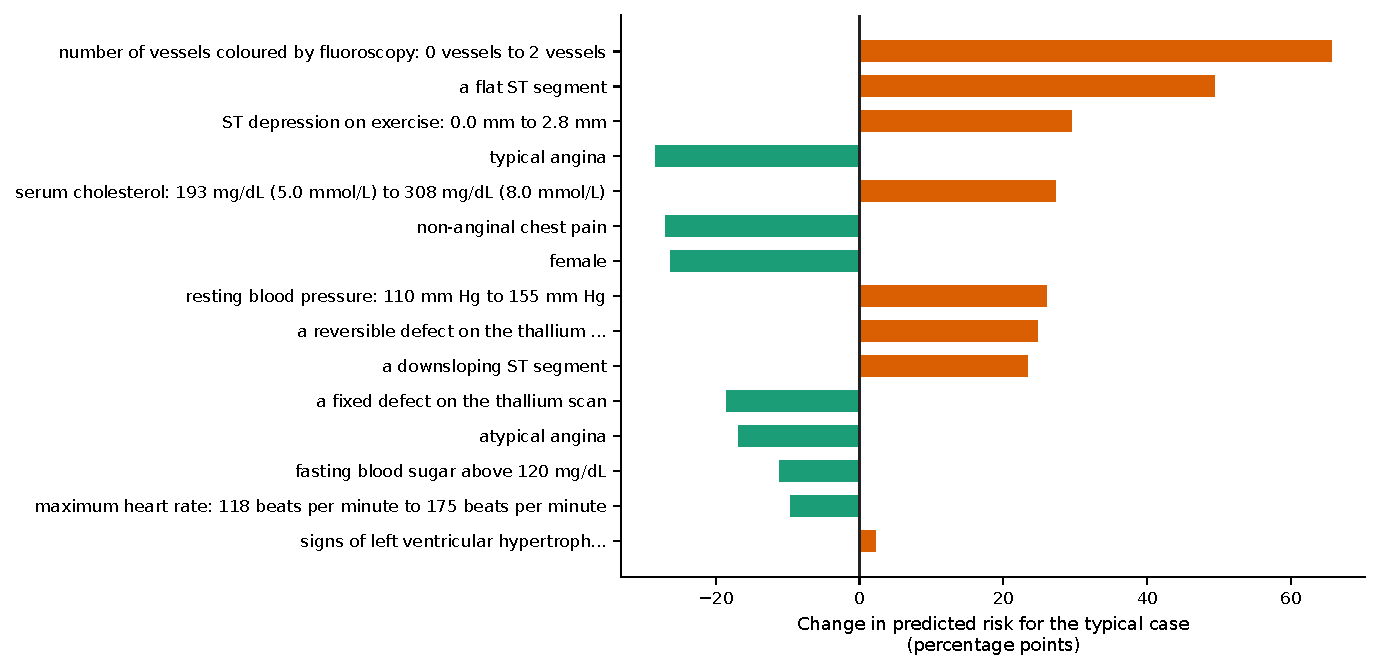
\includegraphics[width=\linewidth,height=0.88\textheight,keepaspectratio]{figures/heart-s2-c3/ann_33-effects.pdf}
\caption{The whole model: Each input's change in the predicted value for the typical case across the whole model, largest first (orange: raises it, teal: lowers it).}
\label{fig:hearts2c3:plot-ann33-0}
\end{figure}
\par\smallskip\noindent{\small \textbf{Dive deeper:} Non-anginal chest pain with heart rate (\ref{rd:ann30}); Non-anginal chest pain with cholesterol (\ref{rd:ann32}); ST depression gate with little effect (\ref{rd:ann31}). Technical detail: \ref{tech:ann33}.\par}
\subsubsection{Non-anginal chest pain with heart rate}\label{rd:ann30}
\noindent{\footnotesize Part of: The whole model (\ref{rd:ann33}).\par}
\noindent{\small Figure~\ref{fig:hearts2c3:parts-ann30} shows what feeds this part; Figure~\ref{fig:hearts2c3:units-ann30} its units and every connection into them (dashed boxes: connections from or to other parts, drawn in their own sections).\par}
\begin{figure}[H]\centering
\resizebox{!}{\ifdim\height>0.5\textheight 0.5\textheight\else\height\fi}{%
\resizebox{\ifdim\width>\linewidth\linewidth\else\width\fi}{!}{%
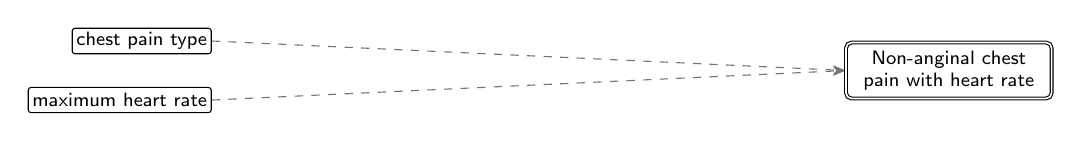
\begin{tikzpicture}[
  font=\sffamily\scriptsize, >={Stealth[length=1.6mm]},
  inp/.style={draw, rounded corners=1pt, fill=white, inner sep=1.5pt, minimum height=3.2mm, anchor=east},
  abox/.style={draw, thick, rounded corners=2pt, align=center, inner sep=3pt, minimum height=6mm, text width=42mm},
  outp/.style={draw, double, rounded corners=2pt, fill=white, align=center, inner sep=3pt, text width=24mm},
  agg/.style={draw=black!55},
]
\node[inp] (i0) at (0,0.375) {chest pain type};
\node[inp] (i1) at (0,-0.375) {maximum heart rate};
\node[outp] (out) at (9.36,0) {Non-anginal chest pain with heart rate};
\begin{scope}[on background layer]
\draw[->, agg, thin, dashed] (i0.east) -- (out.west);
\draw[->, agg, thin, dashed] (i1.east) -- (out.west);
\end{scope}
\end{tikzpicture}}}%
\caption{Non-anginal chest pain with heart rate: what feeds it, one level down.}
\label{fig:hearts2c3:parts-ann30}
\end{figure}
\begin{figure}[H]\centering
\resizebox{\ifdim\width>\linewidth\linewidth\else\width\fi}{!}{%
\definecolor{netup}{HTML}{D95F02}\definecolor{netdown}{HTML}{1B9E77}\definecolor{netmixed}{HTML}{7F7F7F}%
\begin{tikzpicture}[
  font=\sffamily\scriptsize, >={Stealth[length=1.4mm]},
  inp/.style={draw, circle, fill=white, minimum size=3.2mm, inner sep=0pt},
  hid/.style={draw, circle, fill=white, minimum size=5.2mm, inner sep=0.5pt, font=\sffamily\tiny},
  exitbox/.style={draw, thick, rectangle, fill=white, align=center, text width=17mm, minimum height=5mm, inner sep=1.5pt, font=\sffamily\tiny},
  sumbox/.style={draw, thick, dashed, rectangle, fill=white, align=center, text width=17mm, minimum height=5mm, inner sep=1.5pt, font=\sffamily\tiny},
  outp/.style={draw, thick, regular polygon, regular polygon sides=6, fill=white, minimum size=10mm, inner sep=0pt, font=\sffamily\tiny, align=center},
  stub/.style={draw, dashed, rounded corners=2pt, fill=white, align=center, inner sep=2pt, font=\sffamily\tiny, text width=15mm},
  inlab/.style={font=\sffamily\tiny, align=center, text width=15mm, inner sep=1pt, fill=white, fill opacity=0.8, text opacity=1},
  wpos/.style={draw=NavyBlue}, wneg/.style={draw=BrickRed}, wagg/.style={draw=black!45, line width=1.2pt},
  wmix/.style={draw=Plum},
]
\node[exitbox] (n2472) at (3.8,1.9) {Non-anginal chest pain with heart rate $\downarrow$};
\node[inp, draw=netdown, very thick] (ninxxcpx3) at (4.7,0.0) {};
\path (ninxxcpx3.south) node[inlab, anchor=north] (labninxxcpx3) {non-anginal pain $\downarrow$};
\node[inp, draw=netdown, very thick] (ninxxthalach) at (2.9,0.0) {};
\path (ninxxthalach.south) node[inlab, anchor=north] (labninxxthalach) {max heart rate $\downarrow$};
\node[stub] (ntoxxthexmodelxoutput) at (3.8,3.45) {to the model output};
\begin{scope}[on background layer]
\node[fit=(n2472) , inner sep=8pt, rounded corners=5pt, fill=BurntOrange!10, draw=BurntOrange!45] (clu0) {};
\draw[->, wpos, line width=0.63pt] (ninxxcpx3) -- (n2472);
\draw[->, wpos, line width=0.49pt] (ninxxthalach) -- (n2472);
\draw[->, wneg, line width=0.43pt] (n2472) -- (ntoxxthexmodelxoutput);
\end{scope}
\node[font=\sffamily\scriptsize\bfseries, text=BurntOrange!55!black, anchor=south west, inner sep=1pt, fill=white, fill opacity=0.85, text opacity=1] at (clu0.north west) {Non-anginal chest pain with heart rate};
\end{tikzpicture}}%
\caption{Non-anginal chest pain with heart rate: its units and every connection into them. Blue: positive weight (raises the score); red: negative weight (lowers it); thicker: larger weight. Orange outline and up arrow: raises the final prediction; teal and down arrow: lowers it; grey and double arrow: depends.}
\label{fig:hearts2c3:units-ann30}
\end{figure}
\paragraph{Hypothesis.} This part lowers the predicted risk for patients with non-anginal chest pain, and for them a higher maximum heart rate lowers it further, slowly at first, then faster.\,{\scriptsize\textcolor{NavyBlue}{[C30, C32]}}
\paragraph{Evidence.} It acts on 76 of 242 training patients, mostly patients with non-anginal chest pain, 15 of whom had heart disease; for the typical patient it acts on, the predicted risk is about 5\% without it and about 2\% with it.\,{\scriptsize\textcolor{NavyBlue}{[C34]}} Through it, non-anginal chest pain rather than any other chest pain type takes a typical patient's predicted risk from about 30\% to about 17\%.\,{\scriptsize\textcolor{NavyBlue}{[C30]}} Through it, a higher maximum heart rate lowers the risk in an uneven way, for the typical patient it acts on from about 4\% at 118 to about 2\% at 175 beats per minute, flattening out near the bottom because the predicted risk cannot go much lower.\,{\scriptsize\textcolor{NavyBlue}{[C31]}} Across the whole model, a higher maximum heart rate lowers the risk slowly at first, then faster, from about 7\% to about 2\% with non-anginal chest pain, against about 36\% to about 27\% for other chest pain types.\,{\scriptsize\textcolor{NavyBlue}{[C32]}} Its formula reproduces the part exactly on all 242 training patients.\,{\scriptsize\textcolor{NavyBlue}{[C35]}}
\par\noindent{\small Evidence plots: Figure~\ref{fig:hearts2c3:plot-ann30-0}, Figure~\ref{fig:hearts2c3:plot-ann30-1}, Figure~\ref{fig:hearts2c3:plot-ann30-2}, Figure~\ref{fig:hearts2c3:plot-ann30-3}, Figure~\ref{fig:hearts2c3:plot-ann30-4}.\par}
\par\noindent{\small Figure~\ref{fig:hearts2c3:plot-ann30-3} shows this part's own output, unit h1: it switches on at about 184.3 beats per minute of maximum heart rate, and is zero below.\par}
\begin{figure}[H]\centering
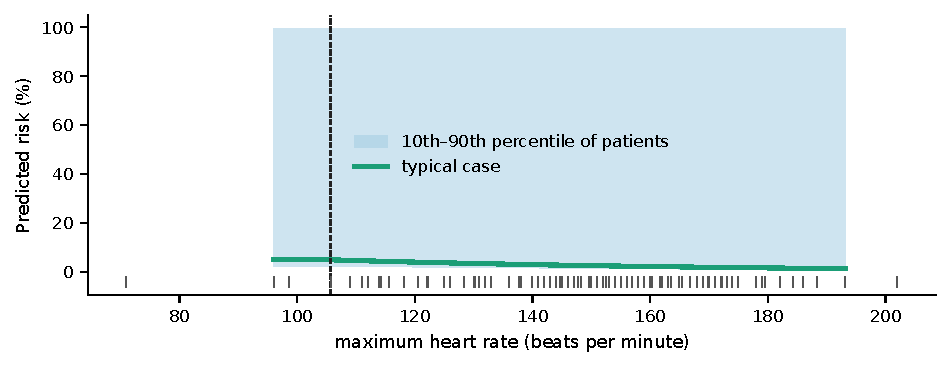
\includegraphics[width=\linewidth,height=0.88\textheight,keepaspectratio]{figures/heart-s2-c3/ann_30-response.pdf}
\caption{Non-anginal chest pain with heart rate: Response curves through this part: the typical case (bold), the 10th to 90th percentile of individual patients (band), the fold or step point (dashed) with its spread across them (grey), and the observed values (ticks).}
\label{fig:hearts2c3:plot-ann30-0}
\end{figure}
\begin{figure}[H]\centering
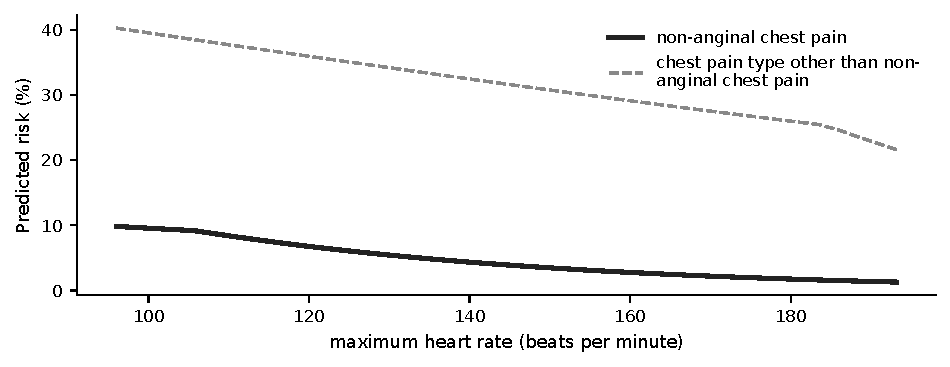
\includegraphics[width=\linewidth,height=0.88\textheight,keepaspectratio]{figures/heart-s2-c3/ann_30-interaction.pdf}
\caption{Non-anginal chest pain with heart rate: How the effect differs between groups: one curve per group, for the typical case of each group.}
\label{fig:hearts2c3:plot-ann30-1}
\end{figure}
\begin{figure}[H]\centering
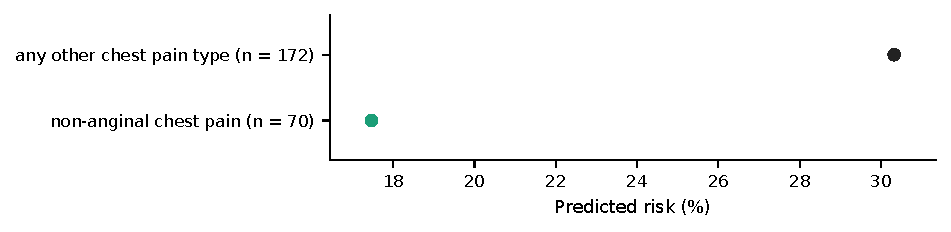
\includegraphics[width=\linewidth,height=0.88\textheight,keepaspectratio]{figures/heart-s2-c3/ann_30-categories-small.pdf}
\caption{Non-anginal chest pain with heart rate: The predicted value for the typical case at each level, through this part (n = training patients; grey: fewer than 20).}
\label{fig:hearts2c3:plot-ann30-2}
\end{figure}
\begin{figure}[H]\centering
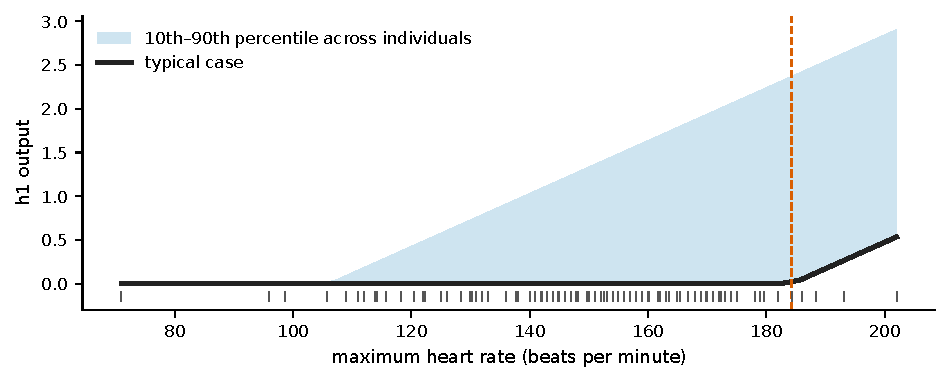
\includegraphics[width=\linewidth,height=0.88\textheight,keepaspectratio]{figures/heart-s2-c3/ann_30-partial-2472.pdf}
\caption{Non-anginal chest pain with heart rate: This part's own output, unit h1 (the output of 'Non-anginal chest pain with heart rate'), on its own scale (its activation), with every other input at the typical case; it is active for 76 of 242. Bold: the typical case; band: 10th to 90th percentile across individuals; dashed: where it switches on; ticks: the data.}
\label{fig:hearts2c3:plot-ann30-3}
\end{figure}
\begin{figure}[H]\centering
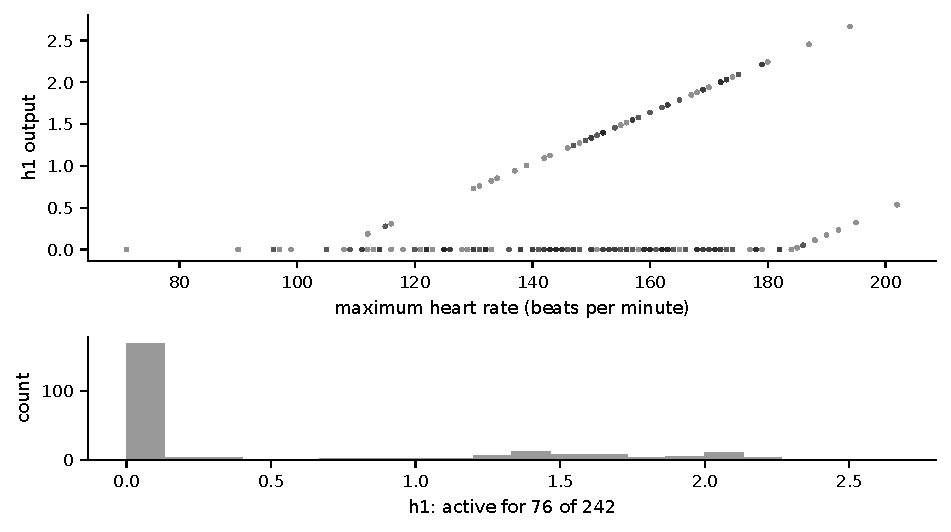
\includegraphics[width=\linewidth,height=0.88\textheight,keepaspectratio]{figures/heart-s2-c3/ann_30-units.pdf}
\caption{Non-anginal chest pain with heart rate: This part's hidden units: each unit's output against its main numeric input (top) and how often it is active (bottom).}
\label{fig:hearts2c3:plot-ann30-4}
\end{figure}
\par\smallskip\noindent{\small Technical detail: \ref{tech:ann30}.\par}
\subsubsection{Non-anginal chest pain with cholesterol}\label{rd:ann32}
\noindent{\footnotesize Part of: The whole model (\ref{rd:ann33}).\par}
\noindent{\small Figure~\ref{fig:hearts2c3:parts-ann32} shows what feeds this part; Figure~\ref{fig:hearts2c3:units-ann32} its units and every connection into them (dashed boxes: connections from or to other parts, drawn in their own sections).\par}
\begin{figure}[H]\centering
\resizebox{!}{\ifdim\height>0.5\textheight 0.5\textheight\else\height\fi}{%
\resizebox{\ifdim\width>\linewidth\linewidth\else\width\fi}{!}{%
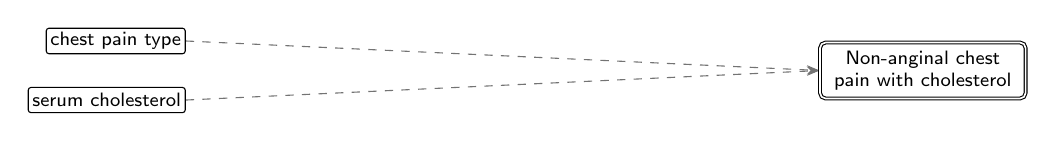
\begin{tikzpicture}[
  font=\sffamily\scriptsize, >={Stealth[length=1.6mm]},
  inp/.style={draw, rounded corners=1pt, fill=white, inner sep=1.5pt, minimum height=3.2mm, anchor=east},
  abox/.style={draw, thick, rounded corners=2pt, align=center, inner sep=3pt, minimum height=6mm, text width=42mm},
  outp/.style={draw, double, rounded corners=2pt, fill=white, align=center, inner sep=3pt, text width=24mm},
  agg/.style={draw=black!55},
]
\node[inp] (i0) at (0,0.375) {chest pain type};
\node[inp] (i1) at (0,-0.375) {serum cholesterol};
\node[outp] (out) at (9.36,0) {Non-anginal chest pain with cholesterol};
\begin{scope}[on background layer]
\draw[->, agg, thin, dashed] (i0.east) -- (out.west);
\draw[->, agg, thin, dashed] (i1.east) -- (out.west);
\end{scope}
\end{tikzpicture}}}%
\caption{Non-anginal chest pain with cholesterol: what feeds it, one level down.}
\label{fig:hearts2c3:parts-ann32}
\end{figure}
\begin{figure}[H]\centering
\resizebox{\ifdim\width>\linewidth\linewidth\else\width\fi}{!}{%
\definecolor{netup}{HTML}{D95F02}\definecolor{netdown}{HTML}{1B9E77}\definecolor{netmixed}{HTML}{7F7F7F}%
\begin{tikzpicture}[
  font=\sffamily\scriptsize, >={Stealth[length=1.4mm]},
  inp/.style={draw, circle, fill=white, minimum size=3.2mm, inner sep=0pt},
  hid/.style={draw, circle, fill=white, minimum size=5.2mm, inner sep=0.5pt, font=\sffamily\tiny},
  exitbox/.style={draw, thick, rectangle, fill=white, align=center, text width=17mm, minimum height=5mm, inner sep=1.5pt, font=\sffamily\tiny},
  sumbox/.style={draw, thick, dashed, rectangle, fill=white, align=center, text width=17mm, minimum height=5mm, inner sep=1.5pt, font=\sffamily\tiny},
  outp/.style={draw, thick, regular polygon, regular polygon sides=6, fill=white, minimum size=10mm, inner sep=0pt, font=\sffamily\tiny, align=center},
  stub/.style={draw, dashed, rounded corners=2pt, fill=white, align=center, inner sep=2pt, font=\sffamily\tiny, text width=15mm},
  inlab/.style={font=\sffamily\tiny, align=center, text width=15mm, inner sep=1pt, fill=white, fill opacity=0.8, text opacity=1},
  wpos/.style={draw=NavyBlue}, wneg/.style={draw=BrickRed}, wagg/.style={draw=black!45, line width=1.2pt},
  wmix/.style={draw=Plum},
]
\node[exitbox] (n2863) at (3.9,1.9) {Non-anginal chest pain with cholesterol $\downarrow$};
\node[inp, draw=netdown, very thick] (ninxxcpx3) at (4.8,0.0) {};
\path (ninxxcpx3.south) node[inlab, anchor=north] (labninxxcpx3) {non-anginal pain $\downarrow$};
\node[inp, draw=netup, very thick] (ninxxchol) at (3.0,0.0) {};
\path (ninxxchol.south) node[inlab, anchor=north] (labninxxchol) {cholesterol $\uparrow$};
\node[stub] (ntoxxthexmodelxoutput) at (3.9,3.45) {to the model output};
\begin{scope}[on background layer]
\node[fit=(n2863) , inner sep=8pt, rounded corners=5pt, fill=ForestGreen!10, draw=ForestGreen!45] (clu0) {};
\draw[->, wpos, line width=0.59pt] (ninxxcpx3) -- (n2863);
\draw[->, wneg, line width=0.38pt] (ninxxchol) -- (n2863);
\draw[->, wneg, line width=0.33pt] (n2863) -- (ntoxxthexmodelxoutput);
\end{scope}
\node[font=\sffamily\scriptsize\bfseries, text=ForestGreen!55!black, anchor=south west, inner sep=1pt, fill=white, fill opacity=0.85, text opacity=1] at (clu0.north west) {Non-anginal chest pain with cholesterol};
\end{tikzpicture}}%
\caption{Non-anginal chest pain with cholesterol: its units and every connection into them. Blue: positive weight (raises the score); red: negative weight (lowers it); thicker: larger weight. Orange outline and up arrow: raises the final prediction; teal and down arrow: lowers it; grey and double arrow: depends.}
\label{fig:hearts2c3:units-ann32}
\end{figure}
\paragraph{Hypothesis.} This part lowers the predicted risk a little further for patients with non-anginal chest pain whose cholesterol stays below about 282 mg/dL.\,{\scriptsize\textcolor{NavyBlue}{[C40, C39]}}
\paragraph{Evidence.} It acts on 61 of 242 training patients, all of them with non-anginal chest pain, 13 of whom had heart disease; for the typical patient it acts on, the predicted risk is about 3\% without it and about 2\% with it.\,{\scriptsize\textcolor{NavyBlue}{[C40]}} Through it, higher cholesterol raises the predicted risk steadily up to about 282 mg/dL, where the part switches off, then no further: for the typical patient it acts on, from about 2\% at 193 mg/dL to about 3\% at 308 mg/dL.\,{\scriptsize\textcolor{NavyBlue}{[C37, C39]}} Through it, non-anginal chest pain rather than any other chest pain type takes a typical patient's predicted risk from about 30\% to about 29\%.\,{\scriptsize\textcolor{NavyBlue}{[C36]}} Across the whole model, higher cholesterol raises the risk in an uneven way from about 2\% to about 7\% with non-anginal chest pain, against about 21\% to about 48\% for other chest pain types.\,{\scriptsize\textcolor{NavyBlue}{[C38]}} Its formula reproduces the part exactly on all 242 training patients.\,{\scriptsize\textcolor{NavyBlue}{[C41]}}
\par\noindent{\small Evidence plots: Figure~\ref{fig:hearts2c3:plot-ann32-0}, Figure~\ref{fig:hearts2c3:plot-ann32-1}, Figure~\ref{fig:hearts2c3:plot-ann32-2}, Figure~\ref{fig:hearts2c3:plot-ann32-3}, Figure~\ref{fig:hearts2c3:plot-ann32-4}.\par}
\par\noindent{\small Figure~\ref{fig:hearts2c3:plot-ann32-3} shows this part's own output, unit h3.\par}
\begin{figure}[H]\centering
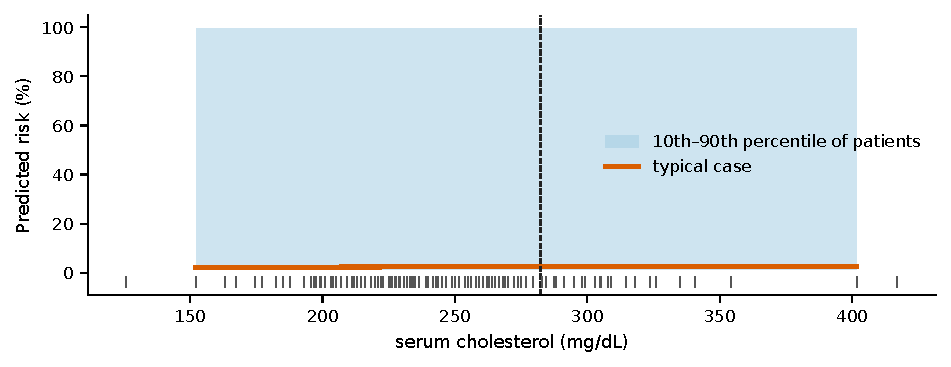
\includegraphics[width=\linewidth,height=0.88\textheight,keepaspectratio]{figures/heart-s2-c3/ann_32-response.pdf}
\caption{Non-anginal chest pain with cholesterol: Response curves through this part: the typical case (bold), the 10th to 90th percentile of individual patients (band), the fold or step point (dashed) with its spread across them (grey), and the observed values (ticks).}
\label{fig:hearts2c3:plot-ann32-0}
\end{figure}
\begin{figure}[H]\centering
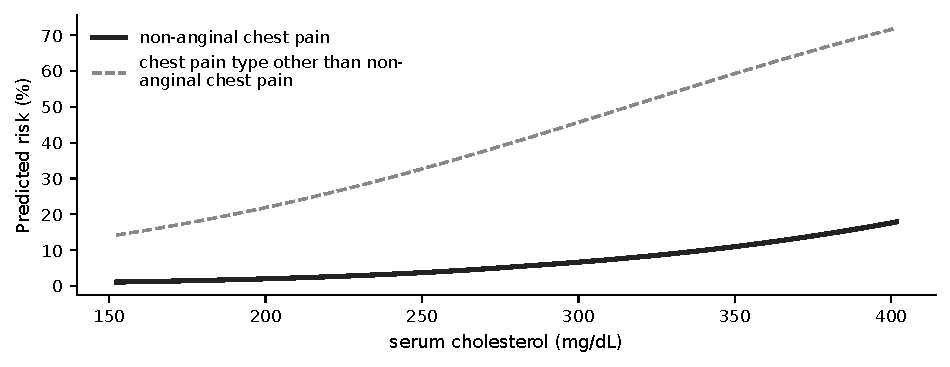
\includegraphics[width=\linewidth,height=0.88\textheight,keepaspectratio]{figures/heart-s2-c3/ann_32-interaction.pdf}
\caption{Non-anginal chest pain with cholesterol: How the effect differs between groups: one curve per group, for the typical case of each group.}
\label{fig:hearts2c3:plot-ann32-1}
\end{figure}
\begin{figure}[H]\centering
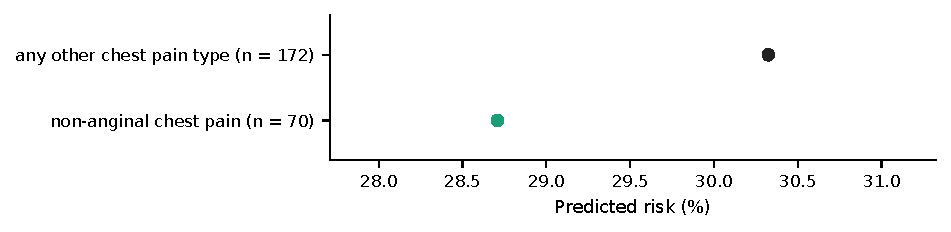
\includegraphics[width=\linewidth,height=0.88\textheight,keepaspectratio]{figures/heart-s2-c3/ann_32-categories-small.pdf}
\caption{Non-anginal chest pain with cholesterol: The predicted value for the typical case at each level, through this part (n = training patients; grey: fewer than 20).}
\label{fig:hearts2c3:plot-ann32-2}
\end{figure}
\begin{figure}[H]\centering
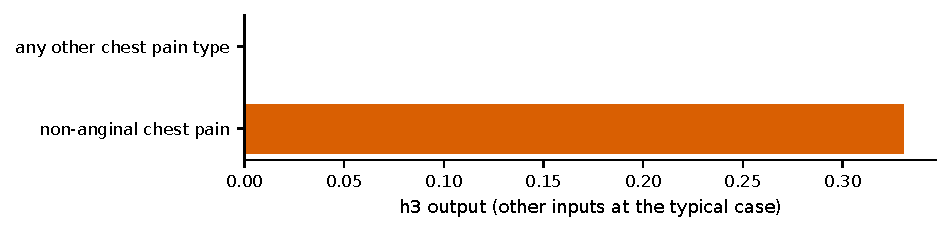
\includegraphics[width=\linewidth,height=0.88\textheight,keepaspectratio]{figures/heart-s2-c3/ann_32-partial-2863.pdf}
\caption{Non-anginal chest pain with cholesterol: This part's own output, unit h3 (the output of 'Non-anginal chest pain with cholesterol'), on its own scale (its activation), with every other input at the typical case; it is active for 61 of 242. Its output for each combination of the levels it reads.}
\label{fig:hearts2c3:plot-ann32-3}
\end{figure}
\begin{figure}[H]\centering
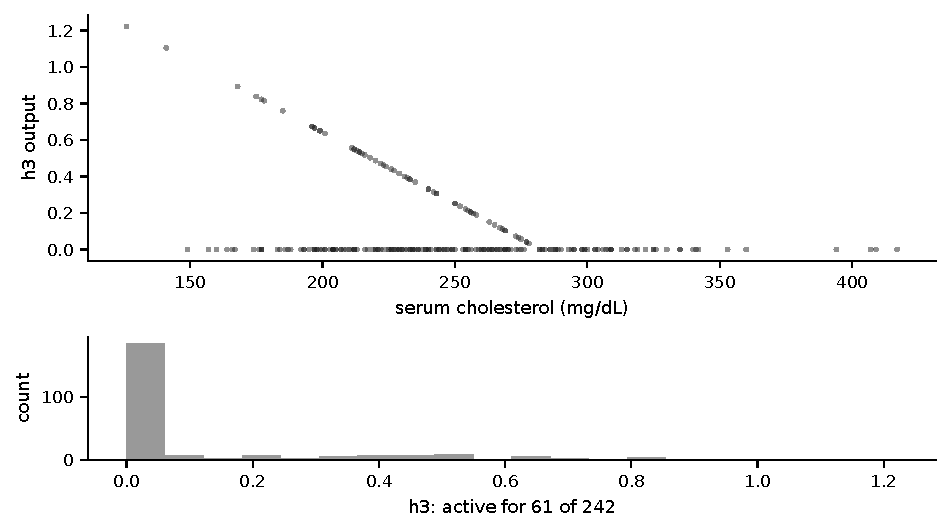
\includegraphics[width=\linewidth,height=0.88\textheight,keepaspectratio]{figures/heart-s2-c3/ann_32-units.pdf}
\caption{Non-anginal chest pain with cholesterol: This part's hidden units: each unit's output against its main numeric input (top) and how often it is active (bottom).}
\label{fig:hearts2c3:plot-ann32-4}
\end{figure}
\par\smallskip\noindent{\small Technical detail: \ref{tech:ann32}.\par}
\subsubsection{ST depression gate with little effect}\label{rd:ann31}
\noindent{\footnotesize Part of: The whole model (\ref{rd:ann33}).\par}
\noindent{\small Figure~\ref{fig:hearts2c3:parts-ann31} shows what feeds this part; Figure~\ref{fig:hearts2c3:units-ann31} its units and every connection into them (dashed boxes: connections from or to other parts, drawn in their own sections).\par}
\begin{figure}[H]\centering
\resizebox{!}{\ifdim\height>0.5\textheight 0.5\textheight\else\height\fi}{%
\resizebox{\ifdim\width>\linewidth\linewidth\else\width\fi}{!}{%
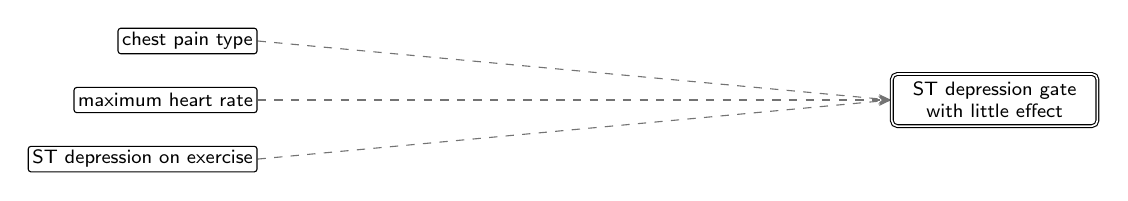
\begin{tikzpicture}[
  font=\sffamily\scriptsize, >={Stealth[length=1.6mm]},
  inp/.style={draw, rounded corners=1pt, fill=white, inner sep=1.5pt, minimum height=3.2mm, anchor=east},
  abox/.style={draw, thick, rounded corners=2pt, align=center, inner sep=3pt, minimum height=6mm, text width=42mm},
  outp/.style={draw, double, rounded corners=2pt, fill=white, align=center, inner sep=3pt, text width=24mm},
  agg/.style={draw=black!55},
]
\node[inp] (i0) at (0,0.75) {chest pain type};
\node[inp] (i1) at (0,-0.0) {maximum heart rate};
\node[inp] (i2) at (0,-0.75) {ST depression on exercise};
\node[outp] (out) at (9.36,0) {ST depression gate with little effect};
\begin{scope}[on background layer]
\draw[->, agg, thin, dashed] (i0.east) -- (out.west);
\draw[->, agg, thin, dashed] (i1.east) -- (out.west);
\draw[->, agg, thin, dashed] (i2.east) -- (out.west);
\end{scope}
\end{tikzpicture}}}%
\caption{ST depression gate with little effect: what feeds it, one level down.}
\label{fig:hearts2c3:parts-ann31}
\end{figure}
\begin{figure}[H]\centering
\resizebox{\ifdim\width>\linewidth\linewidth\else\width\fi}{!}{%
\definecolor{netup}{HTML}{D95F02}\definecolor{netdown}{HTML}{1B9E77}\definecolor{netmixed}{HTML}{7F7F7F}%
\begin{tikzpicture}[
  font=\sffamily\scriptsize, >={Stealth[length=1.4mm]},
  inp/.style={draw, circle, fill=white, minimum size=3.2mm, inner sep=0pt},
  hid/.style={draw, circle, fill=white, minimum size=5.2mm, inner sep=0.5pt, font=\sffamily\tiny},
  exitbox/.style={draw, thick, rectangle, fill=white, align=center, text width=17mm, minimum height=5mm, inner sep=1.5pt, font=\sffamily\tiny},
  sumbox/.style={draw, thick, dashed, rectangle, fill=white, align=center, text width=17mm, minimum height=5mm, inner sep=1.5pt, font=\sffamily\tiny},
  outp/.style={draw, thick, regular polygon, regular polygon sides=6, fill=white, minimum size=10mm, inner sep=0pt, font=\sffamily\tiny, align=center},
  stub/.style={draw, dashed, rounded corners=2pt, fill=white, align=center, inner sep=2pt, font=\sffamily\tiny, text width=15mm},
  inlab/.style={font=\sffamily\tiny, align=center, text width=15mm, inner sep=1pt, fill=white, fill opacity=0.8, text opacity=1},
  wpos/.style={draw=NavyBlue}, wneg/.style={draw=BrickRed}, wagg/.style={draw=black!45, line width=1.2pt},
  wmix/.style={draw=Plum},
]
\node[exitbox] (n2596) at (3.7,1.9) {ST depression gate with little effect $\downarrow$};
\node[inp, draw=netup, very thick] (ninxxcpx3) at (5.5,0.0) {};
\path (ninxxcpx3.south) node[inlab, anchor=north] (labninxxcpx3) {non-anginal pain $\uparrow$};
\node[inp, draw=netup, very thick] (ninxxthalach) at (3.7,0.0) {};
\path (ninxxthalach.south) node[inlab, anchor=north] (labninxxthalach) {max heart rate $\uparrow$};
\node[inp, draw=netdown, very thick] (ninxxoldpeak) at (1.9,0.0) {};
\path (ninxxoldpeak.south) node[inlab, anchor=north] (labninxxoldpeak) {ST depression $\downarrow$};
\node[stub] (ntoxxthexmodelxoutput) at (3.7,3.45) {to the model output};
\begin{scope}[on background layer]
\node[fit=(n2596) , inner sep=8pt, rounded corners=5pt, fill=Orchid!10, draw=Orchid!45] (clu0) {};
\draw[->, wneg, line width=0.59pt] (ninxxcpx3) -- (n2596);
\draw[->, wneg, line width=0.33pt] (ninxxthalach) -- (n2596);
\draw[->, wpos, line width=0.49pt] (ninxxoldpeak) -- (n2596);
\draw[->, wneg, line width=0.26pt] (n2596) -- (ntoxxthexmodelxoutput);
\end{scope}
\node[font=\sffamily\scriptsize\bfseries, text=Orchid!55!black, anchor=south west, inner sep=1pt, fill=white, fill opacity=0.85, text opacity=1] at (clu0.north west) {ST depression gate with little effect};
\end{tikzpicture}}%
\caption{ST depression gate with little effect: its units and every connection into them. Blue: positive weight (raises the score); red: negative weight (lowers it); thicker: larger weight. Orange outline and up arrow: raises the final prediction; teal and down arrow: lowers it; grey and double arrow: depends.}
\label{fig:hearts2c3:units-ann31}
\end{figure}
\paragraph{Hypothesis.} This part barely changes the predictions.\,{\scriptsize\textcolor{NavyBlue}{[C50]}}
\paragraph{Evidence.} It switches on when ST depression on exercise minus about 0.019 $\times$ the maximum heart rate exceeds about -1.71, which never happens with non-anginal chest pain; 73 of 242 training patients are on, and 79\% of them had heart disease, against 29\% of the others.\,{\scriptsize\textcolor{NavyBlue}{[C52]}} It changes the predicted risk by at most 0.5 percentage points: through it, ST depression on exercise and maximum heart rate barely move a typical patient's predicted risk, which stays at about 30\%.\,{\scriptsize\textcolor{NavyBlue}{[C50, C42, C43]}} Its formula reproduces the part exactly on all 242 training patients.\,{\scriptsize\textcolor{NavyBlue}{[C51]}}
\par\noindent{\small Evidence plots: Figure~\ref{fig:hearts2c3:plot-ann31-0}, Figure~\ref{fig:hearts2c3:plot-ann31-1}, Figure~\ref{fig:hearts2c3:plot-ann31-2}, Figure~\ref{fig:hearts2c3:plot-ann31-3}, Figure~\ref{fig:hearts2c3:plot-ann31-4}, Figure~\ref{fig:hearts2c3:plot-ann31-5}, Figure~\ref{fig:hearts2c3:plot-ann31-6}.\par}
\par\medskip\noindent\textbf{Worked example: reading this part.} Figure~\ref{fig:hearts2c3:plot-ann31-2} maps the part's own output over its main inputs. In the grey region it is switched off and adds nothing; past the black line it switches on, and the colour shows how much it adds to the score. The line is the rule in the claim (C52): it switches on when ST depression on exercise minus about 0.019 $\times$ maximum heart rate exceed about -1.71. 73 of 242 training patients lie on the 'on' side, and 79\% of them had heart disease, against 29\% of the others: the filled points crowd on the 'on' side. Figure~\ref{fig:hearts2c3:plot-ann31-3} cuts the map into slices: the hinge moves as the other input changes, which is what a tilted line means. Figure~\ref{fig:hearts2c3:plot-ann31-4} shows what this does to the final prediction for the typical case.\par
\par\noindent{\small Figure~\ref{fig:hearts2c3:plot-ann31-5} shows this part's own output, unit h2: over its two main inputs, with the line where it switches on.\par}
\begin{figure}[H]\centering
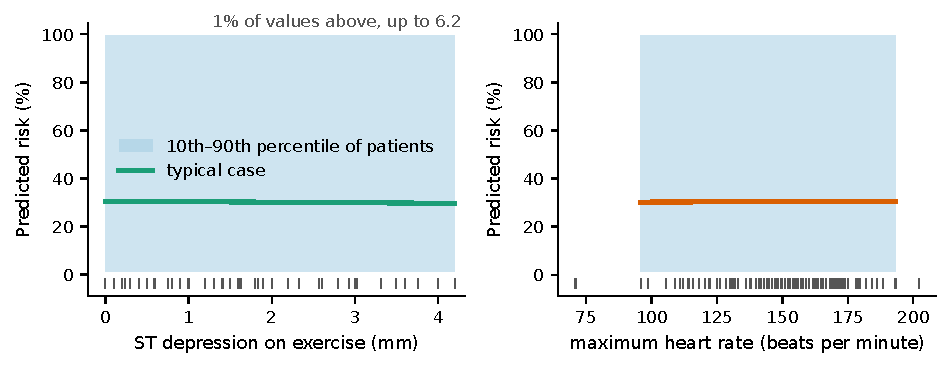
\includegraphics[width=\linewidth,height=0.88\textheight,keepaspectratio]{figures/heart-s2-c3/ann_31-response.pdf}
\caption{ST depression gate with little effect: Response curves through this part: the typical case (bold), the 10th to 90th percentile of individual patients (band), the fold or step point (dashed) with its spread across them (grey), and the observed values (ticks).}
\label{fig:hearts2c3:plot-ann31-0}
\end{figure}
\begin{figure}[H]\centering
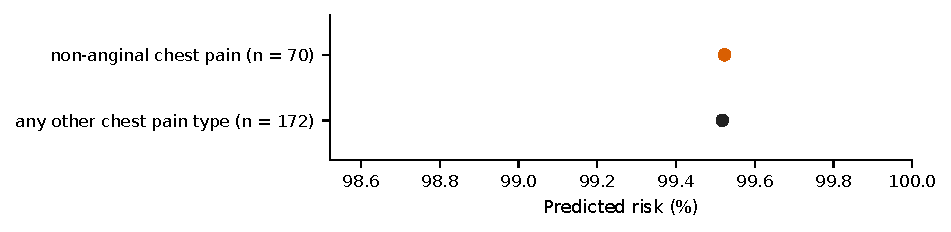
\includegraphics[width=\linewidth,height=0.88\textheight,keepaspectratio]{figures/heart-s2-c3/ann_31-categories-small.pdf}
\caption{ST depression gate with little effect: The predicted value for the typical case at each level, through this part (n = training patients; grey: fewer than 20).}
\label{fig:hearts2c3:plot-ann31-1}
\end{figure}
\begin{figure}[H]\centering
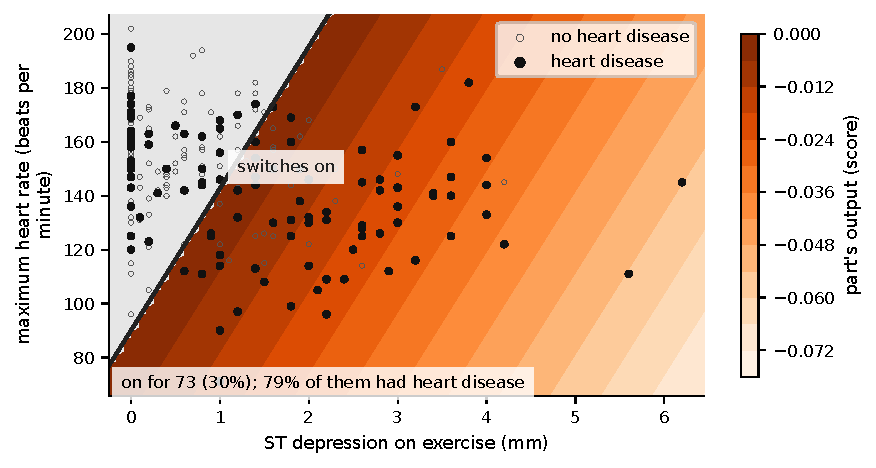
\includegraphics[width=\linewidth,height=0.88\textheight,keepaspectratio]{figures/heart-s2-c3/ann_31-deep-map.pdf}
\caption{ST depression gate with little effect: The part's own output over its two numeric inputs, other inputs at the typical case: colour where it is on, flat grey where it is switched off, the black line where it switches on; training patients as hollow (no event) and filled (event) points, so the part can be seen catching the events (the predicted-chance overlay was harder to read).}
\label{fig:hearts2c3:plot-ann31-2}
\end{figure}
\begin{figure}[H]\centering
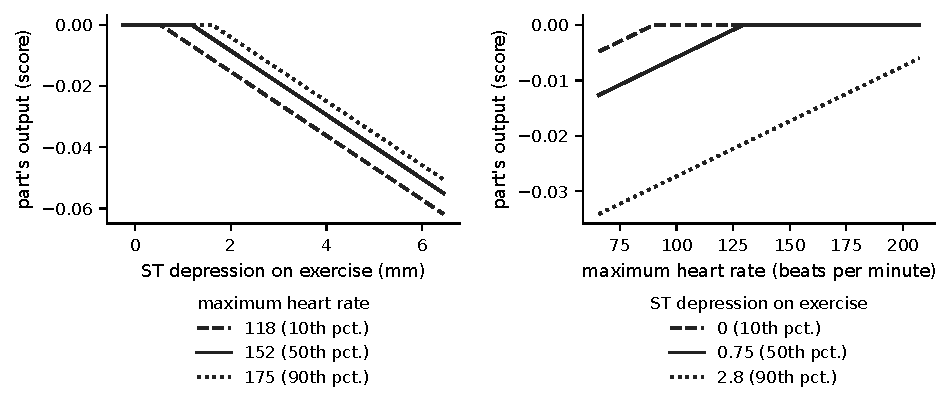
\includegraphics[width=\linewidth,height=0.88\textheight,keepaspectratio]{figures/heart-s2-c3/ann_31-deep-slices.pdf}
\caption{ST depression gate with little effect: Slices of the same map: the part's own output against each input at three values of the other, so the tilted boundary shows as a shifting hinge.}
\label{fig:hearts2c3:plot-ann31-3}
\end{figure}
\begin{figure}[H]\centering
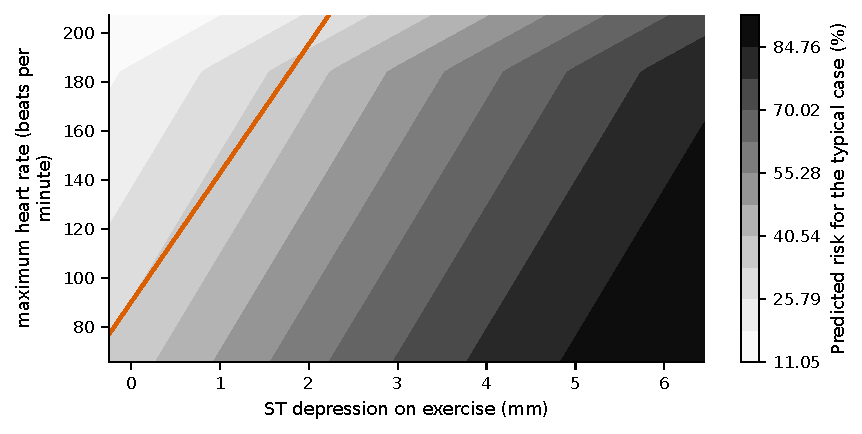
\includegraphics[width=\linewidth,height=0.88\textheight,keepaspectratio]{figures/heart-s2-c3/ann_31-deep-risk.pdf}
\caption{ST depression gate with little effect: The same map on the final scale: the predicted value for the typical case, with the switch-on line (orange).}
\label{fig:hearts2c3:plot-ann31-4}
\end{figure}
\begin{figure}[H]\centering
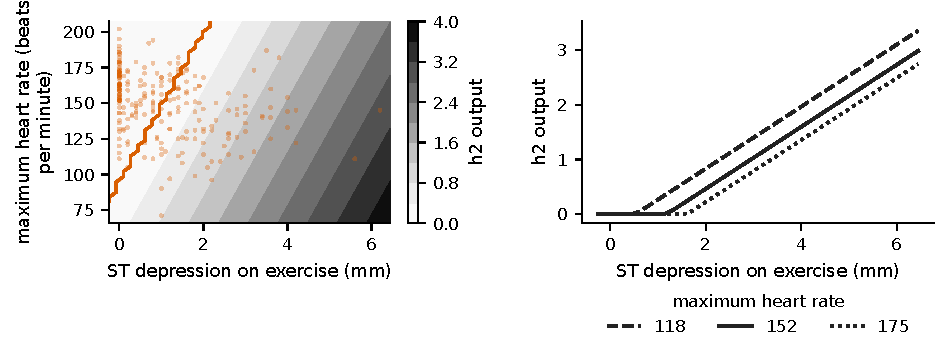
\includegraphics[width=\linewidth,height=0.88\textheight,keepaspectratio]{figures/heart-s2-c3/ann_31-partial-2596.pdf}
\caption{ST depression gate with little effect: This part's own output, unit h2 (the output of 'ST depression gate with little effect'), on its own scale (its activation), with every other input at the typical case; it is active for 73 of 242. Left: its output over its two main inputs (orange line: where it switches on; dots: the data); right: slices at three values of the second input.}
\label{fig:hearts2c3:plot-ann31-5}
\end{figure}
\begin{figure}[H]\centering
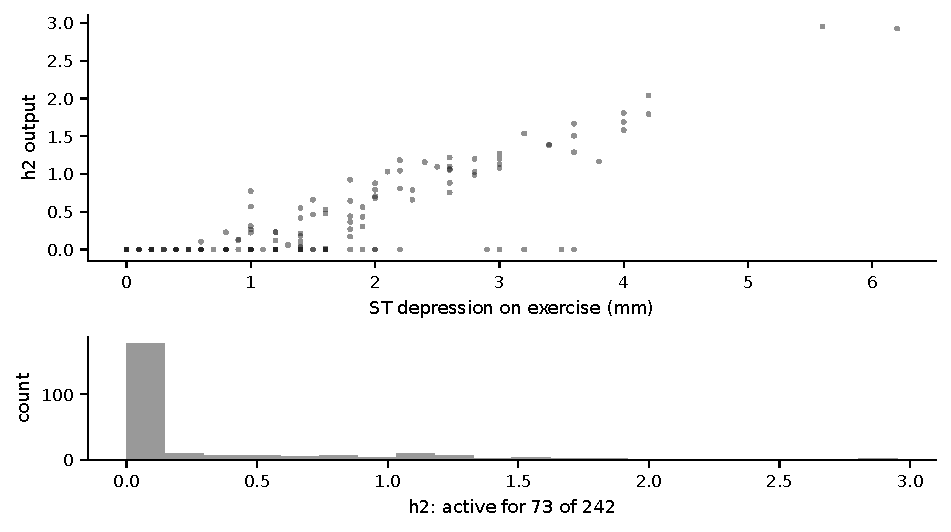
\includegraphics[width=\linewidth,height=0.88\textheight,keepaspectratio]{figures/heart-s2-c3/ann_31-units.pdf}
\caption{ST depression gate with little effect: This part's hidden units: each unit's output against its main numeric input (top) and how often it is active (bottom).}
\label{fig:hearts2c3:plot-ann31-6}
\end{figure}
\par\smallskip\noindent{\small Technical detail: \ref{tech:ann31}.\par}
\subsection{Not supported by the model}
\begin{itemize}\setlength\itemsep{0pt}\small
\item C33: threshold claim about maximum heart rate reached during the exercise test in part ann\_\allowbreak{}30: not supported by the model (the effect past the fold is too small or not consistent across patients).
\item C45: interaction claim about ST depression during exercise (compared with rest) and chest pain type in part ann\_\allowbreak{}31: not supported by the model (the group difference is below 0.1 log-odds).
\item C46: interaction claim about ST depression during exercise (compared with rest) and maximum heart rate reached during the exercise test in part ann\_\allowbreak{}31: not supported by the model (the group difference is below 0.1 log-odds).
\item C47: threshold claim about ST depression during exercise (compared with rest) in part ann\_\allowbreak{}31: not supported by the model (the fold changes the curve by only 0.011 log-odds compared with a straight line (needed 0.1); the effect past the fold is too small or not consistent across patients).
\item C48: threshold claim about maximum heart rate reached during the exercise test in part ann\_\allowbreak{}31: not supported by the model (the fold changes the curve by only 0.022 log-odds compared with a straight line (needed 0.1); the effect past the fold is too small or not consistent across patients).
\item C49: subgroup claim about chest pain type and maximum heart rate reached during the exercise test in part ann\_\allowbreak{}31: not supported by the model (its effect is negligible).
\end{itemize}
\clearpage\section*{Technical detail: heart-s2-c3}
\addcontentsline{toc}{section}{Technical detail: heart-s2-c3}
\noindent{\small The record behind each part: the original hypothesis, the closed form, and every claim with its estimate (log-odds and odds ratio), range across patients, n and test check.\par}
\renewcommand{\thesubsection}{T.\arabic{subsection}}\setcounter{subsection}{0}
\subsection{The whole model}\label{tech:ann33}
\noindent{\footnotesize Annotation ann\_\allowbreak{}33 (heart\_\allowbreak{}disease\_\allowbreak{}logit). Reads: age, sex, chest pain type, resting blood pressure, serum cholesterol, fasting blood sugar, resting ECG, maximum heart rate reached during the exercise test, exercise-induced angina, ST depression during exercise (compared with rest), slope of the ST segment at peak exercise, number of major vessels coloured by fluoroscopy, thallium stress test result.\par}
\paragraph{Original hypothesis (unchanged).} Root: p = sigmoid(z), z = 0.323 + LINEAR CORE - 0.511*\allowbreak{}nonanginal\_\allowbreak{}thalach\_\allowbreak{}gate - 0.018*\allowbreak{}oldpeak\_\allowbreak{}gate\_\allowbreak{}without\_\allowbreak{}nonanginal - 0.235*\allowbreak{}nonanginal\_\allowbreak{}low\_\allowbreak{}chol\_\allowbreak{}gate. LINEAR CORE (16 direct input-$>$output edges, z-scored inputs): ca +1.779, cp:4 +0.869, sex:0 -0.760, slope:2 +0.610, oldpeak +0.559, chol +0.529, thal:7 +0.500, trestbps +0.493, slope:1 -0.488, cp:1 -0.393, sex:1 +0.347, thal:6 -0.282, cp:2 +0.273, fbs:1 -0.209, thalach -0.176, restecg:2 +0.053. Nine inputs are unused (age, fbs:0, restecg:0, restecg:1, exang:0, exang:1, slope:3, thal:3, thal:4; zero-effect entries of this root). Non-anginal pain (cp:3) has no direct edge; it acts only through the three children, all of which are switched by it. COMPOSITION: purely additive in the logit. The children share no hidden nodes and are coupled only through shared inputs (cp:3 feeds all three; thalach, oldpeak and chol also have direct edges). (1) nonanginal\_\allowbreak{}thalach\_\allowbreak{}gate: open for 97\% of non-anginal-pain patients, lowers their risk, more with higher max heart rate; (2) nonanginal\_\allowbreak{}low\_\allowbreak{}chol\_\allowbreak{}gate: open for 87\% of non-anginal-pain patients (those with z-chol $<$ 0.76), lowers their risk more the lower the cholesterol; (3) oldpeak\_\allowbreak{}gate\_\allowbreak{}without\_\allowbreak{}nonanginal: a near-null oldpeak hinge for the other patients (readout -0.018). Together (1)+(2) give non-anginal pain an average logit shift of -0.85 and make thalach and chol slopes depend on chest-pain type. EVIDENCE (train, n=242): full model AUC 0.9381, acc 0.888 (compute\_\allowbreak{}performance)\allowbreak{}. Linear core alone AUC 0.934; logit SD 3.67 (core) vs 0.42 (all nonlinear readouts). Zero-ablating one child at a time: thalach gate 0.934, oldpeak gate 0.938, low-chol gate 0.938. Replacing all hidden readouts with one least-squares linear fit in their four inputs gives 0.938; an L2 logistic regression on all 26 inputs gives 0.936. Mean $|$SHAP$|$ (train, all 242 rows): ca 0.161, cp:4 0.099, sex:0 0.073, slope:2 0.066, thal:7 0.054, slope:1 0.053, oldpeak 0.047, chol 0.041, trestbps 0.040, cp:3 (thalach gate copy) 0.029; unused inputs about 0.001 (estimator noise). Interpretation: logistic regression on 16 inputs plus a non-anginal-pain block whose nonlinearity is small (a linear refit loses nothing on train AUC). Counter-directional signs reported, not explained: cp:2 +0.27 and fbs:1 -0.21 in the core, the low-cholesterol protection for non-anginal pain. Compared with the 10-seed heart-s2 record (key 9083, gen 38, a different cluster of the same run): that genome has an age/\allowbreak{}heart-rate-reserve gate and oldpeak hinges and uses age; this one ignores age entirely and puts its only nonlinear effect on non-anginal chest pain.
\paragraph{Closed form.} Read through its parts (their formulas are in their own sections).
\paragraph{Split inputs.} To annotate the parts, the explanation split these inputs into copies (a refactoring step that does not change what the model computes); the diagrams draw each input once: cholesterol (2 copies); non-anginal pain (3 copies); ST depression (2 copies); max heart rate (3 copies).
\paragraph{Evidence table} (next page, landscape).
\begin{landscape}
{\scriptsize\setlength{\tabcolsep}{3pt}\renewcommand{\arraystretch}{1.15}
\rowcolors{2}{black!6}{white}
\begin{longtable}{@{}l>{\raggedright\arraybackslash}p{0.36\linewidth}>{\raggedright\arraybackslash}p{0.14\linewidth}rrr>{\raggedright\arraybackslash}p{0.06\linewidth}>{\raggedright\arraybackslash}p{0.17\linewidth}c@{}}
\toprule\rowcolor{white}
ID & What is checked & Risk, typical patient & Log-odds & OR & Range (p10--p90) & n & Test check & OK \\
\midrule\endfirsthead
\toprule\rowcolor{white}
ID & What is checked & Risk, typical patient & Log-odds & OR & Range (p10--p90) & n & Test check & OK \\
\midrule\endhead
\bottomrule\endfoot
C01 & direction: number of vessels coloured by fluoroscopy: 0 vessels to 2 vessels (whole model) \newline{\itshape shape: steady (equal steps); 100\% of patients same; verified; risk saturates near 100\%} & 30\% to 96\% & 3.99 & 54.1 & 3.99 to 3.99 & 242 & unclear; AUC gain 0.039 [-0.034, 0.120] & \textcolor{OliveGreen}{yes} \\
C02 & direction: slope of the ST segment at peak exercise: an upsloping ST segment to a flat ST segment (whole model) \newline{\itshape shape: categorical; highest to lowest: a flat ST segment, a downsloping ST segment, an upsloping ST segment} & 30\% to 80\% & 2.20 & 9.04 & 2.20 to 2.20 & 115, 110 & disagrees; AUC gain -0.005 [-0.050, 0.037] & \textcolor{OliveGreen}{yes} \\
C03 & direction: ST depression on exercise: 0.0 mm to 2.8 mm (direct contribution only, not through any part) \newline{\itshape shape: steady; 100\% of patients same; verified} & 23\% to 53\% & 1.32 & 3.74 & 1.32 to 1.32 & 242 & unclear; AUC gain 0.011 [-0.01, 0.038] & \textcolor{OliveGreen}{yes} \\
C04 & direction: ST depression on exercise: 0.0 mm to 2.8 mm (whole model) \newline{\itshape shape: steady; 100\% of patients same; verified} & 23\% to 53\% & 1.31 & 3.69 & 1.30 to 1.32 & 242 & unclear; AUC gain 0.011 [-0.01, 0.038] & \textcolor{OliveGreen}{yes} \\
C05 & direction: chest pain type: no chest pain (asymptomatic) to typical angina (direct contribution only, not through any part) \newline{\itshape shape: categorical; highest to lowest: no chest pain (asymptomatic), atypical angina, non-anginal chest pain, typical angina} & 30\% to 2\% & -3.11 & 0.04 & -3.11 to -3.11 & 108, 22 & agrees; AUC gain 0.038 [0.011, 0.072] & \textcolor{OliveGreen}{yes} \\
C06 & direction: chest pain type: no chest pain (asymptomatic) to typical angina (whole model) \newline{\itshape shape: categorical; highest to lowest: no chest pain (asymptomatic), atypical angina, non-anginal chest pain, typical angina} & 30\% to 2\% & -3.11 & 0.04 & -3.11 to -3.11 & 108, 22 & agrees; AUC gain 0.055 [0.014, 0.101] & \textcolor{OliveGreen}{yes} \\
C07 & direction: serum cholesterol: 193 mg/dL (5.0 mmol/L) to 308 mg/dL (8.0 mmol/L) (direct contribution only, not through any part) \newline{\itshape shape: steady; 100\% of patients same; verified} & 21\% to 48\% & 1.26 & 3.54 & 1.26 to 1.26 & 242 & disagrees; AUC gain -0.012 [-0.044, 0.013] & \textcolor{OliveGreen}{yes} \\
C08 & direction: serum cholesterol: 193 mg/dL (5.0 mmol/L) to 308 mg/dL (8.0 mmol/L) (whole model) \newline{\itshape shape: steady; 100\% of patients same; verified} & 21\% to 48\% & 1.31 & 3.71 & 1.26 to 1.43 & 242 & disagrees; AUC gain -0.012 [-0.044, 0.013] & \textcolor{OliveGreen}{yes} \\
C09 & direction: chest pain type: no chest pain (asymptomatic) to non-anginal chest pain (whole model) \newline{\itshape shape: categorical; highest to lowest: no chest pain (asymptomatic), atypical angina, non-anginal chest pain, typical angina} & 30\% to 3\% & -2.51 & 0.08 & -2.96 to -2.01 & 108, 70 & agrees; AUC gain 0.055 [0.014, 0.101] & \textcolor{OliveGreen}{yes} \\
C10 & direction: sex: male to female (whole model) \newline{\itshape shape: categorical; highest to lowest: male, female} & 30\% to 4\% & -2.33 & 0.10 & -2.33 to -2.33 & 159, 83 & unclear; AUC gain 0.025 [-0.011, 0.071] & \textcolor{OliveGreen}{yes} \\
C11 & direction: resting blood pressure: 110 mm Hg to 155 mm Hg (whole model) \newline{\itshape shape: steady; 100\% of patients same; verified} & 20\% to 46\% & 1.22 & 3.39 & 1.22 to 1.22 & 242 & unclear; AUC gain 0.004 [-0.019, 0.032] & \textcolor{OliveGreen}{yes} \\
C12 & direction: thallium stress test result: thallium stress test result other than a fixed defect on the thallium scan, a reversible defect on the thallium scan to a reversible defect on the thallium scan (whole model) \newline{\itshape shape: categorical; highest to lowest: a reversible defect on the thallium scan, thallium stress test result other than a fixed defect on the thallium scan, a reversible defect on the thallium scan, a fixed defect on the thallium scan} & 30\% to 55\% & 1.03 & 2.81 & 1.03 to 1.03 & 137, 90 & unclear; AUC gain 0.020 [-0.008, 0.054] & \textcolor{OliveGreen}{yes} \\
C13 & direction: slope of the ST segment at peak exercise: an upsloping ST segment to a downsloping ST segment (whole model) \newline{\itshape shape: categorical; highest to lowest: a flat ST segment, a downsloping ST segment, an upsloping ST segment} & 30\% to 54\% & 0.98 & 2.66 & 0.98 to 0.98 & 115, 17 (small n) & disagrees; AUC gain -0.005 [-0.050, 0.037] & \textcolor{OliveGreen}{yes} \\
C14 & direction: chest pain type: no chest pain (asymptomatic) to non-anginal chest pain (direct contribution only, not through any part) \newline{\itshape shape: categorical; highest to lowest: no chest pain (asymptomatic), atypical angina, non-anginal chest pain, typical angina} & 30\% to 7\% & -1.75 & 0.17 & -1.75 to -1.75 & 108, 70 & agrees; AUC gain 0.038 [0.011, 0.072] & \textcolor{OliveGreen}{yes} \\
C15 & direction: thallium stress test result: thallium stress test result other than a fixed defect on the thallium scan, a reversible defect on the thallium scan to a fixed defect on the thallium scan (whole model) \newline{\itshape shape: categorical; highest to lowest: a reversible defect on the thallium scan, thallium stress test result other than a fixed defect on the thallium scan, a reversible defect on the thallium scan, a fixed defect on the thallium scan} & 30\% to 12\% & -1.17 & 0.31 & -1.17 to -1.17 & 137, 15 (small n) & unclear; AUC gain 0.020 [-0.008, 0.054] & \textcolor{OliveGreen}{yes} \\
C16 & direction: chest pain type: no chest pain (asymptomatic) to atypical angina (direct contribution only, not through any part) \newline{\itshape shape: categorical; highest to lowest: no chest pain (asymptomatic), atypical angina, non-anginal chest pain, typical angina} & 30\% to 13\% & -1.03 & 0.36 & -1.03 to -1.03 & 108, 42 & agrees; AUC gain 0.038 [0.011, 0.072] & \textcolor{OliveGreen}{yes} \\
C17 & direction: chest pain type: no chest pain (asymptomatic) to atypical angina (whole model) \newline{\itshape shape: categorical; highest to lowest: no chest pain (asymptomatic), atypical angina, non-anginal chest pain, typical angina} & 30\% to 13\% & -1.03 & 0.36 & -1.03 to -1.03 & 108, 42 & agrees; AUC gain 0.055 [0.014, 0.101] & \textcolor{OliveGreen}{yes} \\
C18 & direction: fasting blood sugar: fasting blood sugar of 120 mg/dL or less to fasting blood sugar above 120 mg/dL (whole model) \newline{\itshape shape: categorical; highest to lowest: fasting blood sugar of 120 mg/dL or less, fasting blood sugar above 120 mg/dL} & 30\% to 19\% & -0.61 & 0.54 & -0.61 to -0.61 & 209, 33 & unclear; AUC gain 0.001 [-0.012, 0.016] & \textcolor{OliveGreen}{yes} \\
C19 & direction: maximum heart rate: 118 beats per minute to 175 beats per minute (direct contribution only, not through any part) \newline{\itshape shape: steady; 100\% of patients same; verified} & 36\% to 27\% & -0.45 & 0.64 & -0.45 to -0.45 & 242 & unclear; AUC gain 0.005 [-0.004, 0.020] & \textcolor{OliveGreen}{yes} \\
C20 & direction: maximum heart rate: 118 beats per minute to 175 beats per minute (whole model) \newline{\itshape shape: accelerating; 100\% of patients same; verified} & 36\% to 27\% & -0.70 & 0.50 & -1.33 to -0.44 & 242 & unclear; AUC gain 0.012 [-0.002, 0.034] & \textcolor{OliveGreen}{yes} \\
C21 & direction: resting ECG: resting ECG other than signs of left ventricular hypertrophy on the resting ECG to signs of left ventricular hypertrophy on the resting ECG (whole model) \newline{\itshape shape: categorical; highest to lowest: signs of left ventricular hypertrophy on the resting ECG, resting ECG other than signs of left ventricular hypertrophy on the resting ECG} & 30\% to 33\% & 0.11 & 1.11 & 0.11 to 0.11 & 123, 119 & disagrees; AUC gain -0.002 [-0.010, 0.000] & \textcolor{OliveGreen}{yes} \\
C22 & magnitude: number of vessels coloured by fluoroscopy: 0 vessels to 2 vessels, typical patient \newline{\itshape shape: steady (equal steps); 100\% of patients same; verified; risk saturates near 100\%} & 30\% to 96\% & 3.99 & 54.1 &  & 242 & unclear; AUC gain 0.039 [-0.034, 0.120] & \textcolor{OliveGreen}{yes} \\
C23 & magnitude: slope of the ST segment at peak exercise: an upsloping ST segment to a flat ST segment, typical patient \newline{\itshape shape: categorical; highest to lowest: a flat ST segment, a downsloping ST segment, an upsloping ST segment} & 30\% to 80\% & 2.20 & 9.04 &  & 115, 110 & disagrees; AUC gain -0.005 [-0.050, 0.037] & \textcolor{OliveGreen}{yes} \\
C24 & magnitude: ST depression on exercise: 0.0 mm to 2.8 mm, typical patient \newline{\itshape shape: steady; 100\% of patients same; verified} & 23\% to 53\% & 1.30 & 3.68 &  & 242 & unclear; AUC gain 0.011 [-0.01, 0.038] & \textcolor{OliveGreen}{yes} \\
C25 & magnitude: chest pain type: no chest pain (asymptomatic) to typical angina, typical patient \newline{\itshape shape: categorical; highest to lowest: no chest pain (asymptomatic), atypical angina, non-anginal chest pain, typical angina} & 30\% to 2\% & -3.11 & 0.04 &  & 108, 22 & agrees; AUC gain 0.055 [0.014, 0.101] & \textcolor{OliveGreen}{yes} \\
C26 & magnitude: serum cholesterol: 193 mg/dL (5.0 mmol/L) to 308 mg/dL (8.0 mmol/L), typical patient \newline{\itshape shape: steady; 100\% of patients same; verified} & 21\% to 48\% & 1.26 & 3.54 &  & 242 & disagrees; AUC gain -0.012 [-0.044, 0.013] & \textcolor{OliveGreen}{yes} \\
C27 & null: model ignores age (exact rule) &  & 0.00 &  &  & 242 & train only & \textcolor{OliveGreen}{yes} \\
C28 & null: model ignores exercise-induced angina (exact rule) &  & 0.00 &  &  & 242 & train only & \textcolor{OliveGreen}{yes} \\
C29 & structure: made of nonanginal\_\allowbreak{}thalach\_\allowbreak{}gate,\allowbreak{} oldpeak\_\allowbreak{}gate\_\allowbreak{}without\_\allowbreak{}nonanginal,\allowbreak{} nonanginal\_\allowbreak{}low\_\allowbreak{}chol\_\allowbreak{}gate and inputs sex, cp, trestbps, chol, fbs, restecg, thalach, oldpeak, slope, ca, thal; added &  &  &  &  & 242 & train only & \textcolor{OliveGreen}{yes} \\
\end{longtable}}
\end{landscape}
\subsection{Non-anginal chest pain with heart rate}\label{tech:ann30}
\noindent{\footnotesize Annotation ann\_\allowbreak{}30 (nonanginal\_\allowbreak{}thalach\_\allowbreak{}gate). Reads: chest pain type, maximum heart rate reached during the exercise test.\par}
\paragraph{Original hypothesis (unchanged).} Non-anginal-pain gate (protective). 2472 = ReLU(-0.348 + 1.076*cp:3 + 0.678*thalach), read out -0.511 into the logit. Hypothesis: this gate is how the model gives non-anginal chest pain (cp:3, which has no direct edge) a lower risk: it is open for nearly every non-anginal-pain patient and almost never otherwise, and once open a higher achieved max heart rate lowers the risk further (on top of thalach's small direct -0.176 edge). EVIDENCE (train, n=242): active for 97\% of the 70 non-anginal-pain patients (closed only for z-thalach $<$ -1.97) and 5\% of the 172 others (only z-thalach $>$ 1.53). Disease rate 20\% when active vs 55\% when inactive. For a non-anginal-pain patient it adds -0.684 - 0.346*z-thalach to the logit (mean -0.76). Mean $|$sensitivity$|$ cp:3 0.34 $>$ thalach 0.21. Zero-ablating its readout lowers train AUC 0.938 -$>$ 0.934, the only nonlinear part that matters; a linear refit in (cp:3, thalach) recovers 0.938 (R2 0.87), so the gate acts almost as a cp:3 main effect plus a cp:3-specific thalach slope. Supported.
\paragraph{Closed form} {\footnotesize(weights and biases at 3 significant figures; largest difference from the part on the training patients 4.44089e-16).}
{\small\begingroup\allowdisplaybreaks
\begin{align*}
y_{0} &= \operatorname{relu}\bigl(-0.348 + 1.08 x_{cp:3\_a} + 0.678 x_{thalach\_b}\bigr)
\end{align*}\endgroup}

\paragraph{Evidence table} (next page, landscape).
\begin{landscape}
{\scriptsize\setlength{\tabcolsep}{3pt}\renewcommand{\arraystretch}{1.15}
\rowcolors{2}{black!6}{white}
\begin{longtable}{@{}l>{\raggedright\arraybackslash}p{0.36\linewidth}>{\raggedright\arraybackslash}p{0.14\linewidth}rrr>{\raggedright\arraybackslash}p{0.06\linewidth}>{\raggedright\arraybackslash}p{0.17\linewidth}c@{}}
\toprule\rowcolor{white}
ID & What is checked & Risk, typical patient & Log-odds & OR & Range (p10--p90) & n & Test check & OK \\
\midrule\endfirsthead
\toprule\rowcolor{white}
ID & What is checked & Risk, typical patient & Log-odds & OR & Range (p10--p90) & n & Test check & OK \\
\midrule\endhead
\bottomrule\endfoot
C30 & direction: chest pain type: chest pain type other than non-anginal chest pain to non-anginal chest pain (through this part) \newline{\itshape shape: categorical; highest to lowest: chest pain type other than non-anginal chest pain, non-anginal chest pain} & 30\% to 17\% & -0.69 & 0.50 & -1.07 to -0.19 & 172, 70 & unclear; AUC gain 0.008 [-0.009, 0.028] & \textcolor{OliveGreen}{yes} \\
C31 & direction: maximum heart rate: 118 beats per minute to 175 beats per minute (through this part) \newline{\itshape shape: hinge at 106 beats per minute; 29\% of patients same; fallback; risk saturates near 0\%} & 4\% to 2\% (typical patient this part acts on) & -0.25 & 0.78 & -0.88 to 0.00 & 242 & unclear; AUC gain 0.006 [0.000, 0.020] & \textcolor{OliveGreen}{yes} \\
C32 & interaction: effect of maximum heart rate (118 beats per minute to 175 beats per minute) by chest pain type: non-anginal chest pain minus chest pain type other than non-anginal chest pain; stronger in non-anginal chest pain \newline{\itshape shape: accelerating; 100\% of patients same; verified; risk saturates near 0\%} & non-anginal chest pain: 7\% to 2\%; chest pain type other than non-anginal chest pain: 36\% to 27\% & -0.89 & 0.41 &  & 70, 172 & agrees; AUC gain 0.008 [-0.009, 0.028] & \textcolor{OliveGreen}{yes} \\
C33 & threshold: maximum heart rate: fold at about 184 beats per minute (starts) for patients with no chest pain symptoms (asymptomatic) \newline{\itshape shape: step at 190 beats per minute; 100\% of patients same; verified; risk saturates near 100\%} & 99\% to 99\% (typical patient with a fold (patients with no chest pain symptoms (asymptomatic))) & 0.00 & 1.00 & 0.00 to 0.00 & 108, 3 (small n) & unclear; AUC gain 0.006 [0.000, 0.020] & \textcolor{BrickRed}{no} \\
C34 & subgroup: who this part acts on: 76 of 242 patients & 5\% to 2\% (typical patient this part acts on (risk without the part, then with it)) & -0.71 & 0.49 & -1.06 to -0.14 & 76, 166 & unclear; AUC gain 0.013 [-0.001, 0.038] & \textcolor{OliveGreen}{yes} \\
C35 & structure: its formula reproduces it on 242 training patients (largest difference 4.44089e-16) &  & 4e-16 &  &  & 242 & train only & \textcolor{OliveGreen}{yes} \\
\end{longtable}}
\end{landscape}
\subsection{Non-anginal chest pain with cholesterol}\label{tech:ann32}
\noindent{\footnotesize Annotation ann\_\allowbreak{}32 (nonanginal\_\allowbreak{}low\_\allowbreak{}chol\_\allowbreak{}gate). Reads: chest pain type, serum cholesterol.\par}
\paragraph{Original hypothesis (unchanged).} Non-anginal-pain, low-cholesterol gate (protective, small). 2863 = ReLU(-1.255 + 0.983*cp:3 - 0.376*chol), read out -0.235. Hypothesis: open only for non-anginal-pain patients whose cholesterol is not high (z-chol below 0.76); it lowers their risk, by more the lower the cholesterol, so for these patients cholesterol's direct +0.529 edge is partly undone. EVIDENCE (train, n=242): active for 87\% of the 70 non-anginal-pain patients and none of the others. Disease rate 21\% when active vs 52\% when inactive. Readout up to -0.29 logit units (SD 0.053). Mean $|$sensitivity$|$ cp:3 0.25 $>$ chol 0.09. Zero-ablating it leaves train AUC unchanged (0.9381 -$>$ 0.9382): it shifts the level of the non-anginal-pain group rather than ranking patients. Supported but small.
\paragraph{Closed form} {\footnotesize(weights and biases at 3 significant figures; largest difference from the part on the training patients 2.22045e-16).}
{\small\begingroup\allowdisplaybreaks
\begin{align*}
y_{0} &= \operatorname{relu}\bigl(-1.25 + 0.983 x_{cp:3\_c} - 0.376 x_{chol\_b}\bigr)
\end{align*}\endgroup}

\paragraph{Evidence table} (next page, landscape).
\begin{landscape}
{\scriptsize\setlength{\tabcolsep}{3pt}\renewcommand{\arraystretch}{1.15}
\rowcolors{2}{black!6}{white}
\begin{longtable}{@{}l>{\raggedright\arraybackslash}p{0.36\linewidth}>{\raggedright\arraybackslash}p{0.14\linewidth}rrr>{\raggedright\arraybackslash}p{0.06\linewidth}>{\raggedright\arraybackslash}p{0.17\linewidth}c@{}}
\toprule\rowcolor{white}
ID & What is checked & Risk, typical patient & Log-odds & OR & Range (p10--p90) & n & Test check & OK \\
\midrule\endfirsthead
\toprule\rowcolor{white}
ID & What is checked & Risk, typical patient & Log-odds & OR & Range (p10--p90) & n & Test check & OK \\
\midrule\endhead
\bottomrule\endfoot
C36 & direction: chest pain type: chest pain type other than non-anginal chest pain to non-anginal chest pain (through this part) \newline{\itshape shape: categorical; highest to lowest: chest pain type other than non-anginal chest pain, non-anginal chest pain} & 30\% to 29\% & -0.08 & 0.92 & -0.16 to 0.00 & 172, 70 & unclear; AUC gain 0.002 [0.000, 0.009] & \textcolor{OliveGreen}{yes} \\
C37 & direction: serum cholesterol: 193 mg/dL (5.0 mmol/L) to 308 mg/dL (8.0 mmol/L) (through this part) \newline{\itshape shape: hinge at 282 mg/dL (7.3 mmol/L); 100\% of patients same; verified; risk saturates near 0\%; one point with C39 (median fold 282 mg/dL (7.3 mmol/L), typical patient 283 mg/dL (7.3 mmol/L), 10th-90th percentile 282 mg/dL (7.3 mmol/L) to 282 mg/dL (7.3 mmol/L))} & 2\% to 3\% (typical patient this part acts on) & 0.05 & 1.05 & 0.00 to 0.16 & 242 & disagrees; AUC gain -0.001 [-0.006, 0.000] & \textcolor{OliveGreen}{yes} \\
C38 & interaction: effect of serum cholesterol (193 mg/dL (5.0 mmol/L) to 308 mg/dL (8.0 mmol/L)) by chest pain type: non-anginal chest pain minus chest pain type other than non-anginal chest pain; stronger in non-anginal chest pain \newline{\itshape shape: steady; 100\% of patients same; fallback; risk saturates near 0\%} & non-anginal chest pain: 2\% to 7\%; chest pain type other than non-anginal chest pain: 21\% to 48\% & 0.16 & 1.18 &  & 70, 172 & agrees; AUC gain 0.002 [0.000, 0.009] & \textcolor{OliveGreen}{yes} \\
C39 & threshold: serum cholesterol: fold at about 282 mg/dL (7.3 mmol/L) (stops) for patients with non-anginal chest pain \newline{\itshape shape: hinge at 282 mg/dL (7.3 mmol/L); 100\% of patients same; verified; risk saturates near 0\%; one point with C39 (median fold 282 mg/dL (7.3 mmol/L), typical patient 283 mg/dL (7.3 mmol/L), 10th-90th percentile 282 mg/dL (7.3 mmol/L) to 282 mg/dL (7.3 mmol/L))} & 2\% to 3\% (typical patient with a fold) & 0.19 & 1.21 & 0.19 to 0.19 & 70, 61 & disagrees; AUC gain -0.001 [-0.006, 0.000] & \textcolor{OliveGreen}{yes} \\
C40 & subgroup: who this part acts on: 61 of 242 patients & 3\% to 2\% (typical patient this part acts on (risk without the part, then with it)) & -0.10 & 0.91 & -0.18 to -0.02 & 61, 181 & unclear; AUC gain 0.000 [0.000, 0.000] & \textcolor{OliveGreen}{yes} \\
C41 & structure: its formula reproduces it on 242 training patients (largest difference 2.22045e-16) &  & 2e-16 &  &  & 242 & train only & \textcolor{OliveGreen}{yes} \\
\end{longtable}}
\end{landscape}
\subsection{ST depression gate with little effect}\label{tech:ann31}
\noindent{\footnotesize Annotation ann\_\allowbreak{}31 (oldpeak\_\allowbreak{}gate\_\allowbreak{}without\_\allowbreak{}nonanginal). Reads: chest pain type, maximum heart rate reached during the exercise test, ST depression during exercise (compared with rest).\par}
\paragraph{Original hypothesis (unchanged).} ST-depression gate for patients without non-anginal pain (negligible). 2596 = ReLU(-0.688 - 0.985*cp:3 - 0.241*thalach + 0.673*oldpeak), read out -0.018. Hypothesis: a hinge on ST depression (and lower max heart rate) for patients without non-anginal pain, whose readout is too small to change predictions. EVIDENCE (train, n=242): active for 42\% of patients without non-anginal pain and never with it; disease rate 80\% when active vs 29\% when inactive, so it tracks risk, but its readout has SD 0.009 logit units against 3.67 for the linear core, and removing it changes train AUC by +0.0001. Its sign (slightly lowering the risk with more ST depression) runs against oldpeak's direct +0.559 edge, which dominates. Supported as a near-null part; a vestige rather than a mechanism.
\paragraph{Closed form} {\footnotesize(weights and biases at 3 significant figures; largest difference from the part on the training patients 2.22045e-16).}
{\small\begingroup\allowdisplaybreaks
\begin{align*}
y_{0} &= \operatorname{relu}\bigl(-0.688 + 0.673 x_{oldpeak\_b} - 0.241 x_{thalach\_c} \\
&\qquad - 0.985 x_{cp:3\_b}\bigr)
\end{align*}\endgroup}

\paragraph{Evidence table} (next page, landscape).
\begin{landscape}
{\scriptsize\setlength{\tabcolsep}{3pt}\renewcommand{\arraystretch}{1.15}
\rowcolors{2}{black!6}{white}
\begin{longtable}{@{}l>{\raggedright\arraybackslash}p{0.36\linewidth}>{\raggedright\arraybackslash}p{0.14\linewidth}rrr>{\raggedright\arraybackslash}p{0.06\linewidth}>{\raggedright\arraybackslash}p{0.17\linewidth}c@{}}
\toprule\rowcolor{white}
ID & What is checked & Risk, typical patient & Log-odds & OR & Range (p10--p90) & n & Test check & OK \\
\midrule\endfirsthead
\toprule\rowcolor{white}
ID & What is checked & Risk, typical patient & Log-odds & OR & Range (p10--p90) & n & Test check & OK \\
\midrule\endhead
\bottomrule\endfoot
C42 & direction: ST depression on exercise: 0.0 mm to 2.8 mm (through this part) \newline{\itshape shape: flat; 100\% of patients same; verified} & 30\% to 30\% & -0.01 & 0.99 & -0.02 to 0.00 & 242 & unclear; AUC gain 0.000 [0.000, 0.000] & \textcolor{OliveGreen}{yes} \\
C43 & direction: maximum heart rate: 118 beats per minute to 175 beats per minute (through this part) \newline{\itshape shape: flat; 100\% of patients same; verified} & 30\% to 30\% & 0.004 & 1.00 & 0.00 to 0.01 & 242 & unclear; AUC gain 0.000 [0.000, 0.000] & \textcolor{OliveGreen}{yes} \\
C44 & direction: chest pain type: chest pain type other than non-anginal chest pain to non-anginal chest pain (through this part) \newline{\itshape shape: categorical; highest to lowest: non-anginal chest pain, chest pain type other than non-anginal chest pain} & $>$99\% to $>$99\% (typical patient this part acts on) & 0.005 & 1.01 & 0.00 to 0.02 & 172, 70 & unclear; AUC gain 0.000 [0.000, 0.000] & \textcolor{OliveGreen}{yes} \\
C45 & interaction: effect of ST depression on exercise (0.0 mm to 2.8 mm) by chest pain type: non-anginal chest pain minus chest pain type other than non-anginal chest pain; stronger in non-anginal chest pain \newline{\itshape shape: steady; 100\% of patients same; verified; risk saturates near 0\%} & non-anginal chest pain: 2\% to 8\%; chest pain type other than non-anginal chest pain: 23\% to 53\% & 0.02 & 1.02 &  & 70, 172 & agrees; AUC gain 0.000 [0.000, 0.000] & \textcolor{BrickRed}{no} \\
C46 & interaction: effect of ST depression on exercise (0.0 mm to 2.8 mm) by maximum heart rate: maximum heart rate above 152 beats per minute minus maximum heart rate at or below 152 beats per minute; stronger in maximum heart rate above 152 beats per minute \newline{\itshape shape: steady; 100\% of patients same; verified} & maximum heart rate above 152 beats per minute: 21\% to 50\%; maximum heart rate at or below 152 beats per minute: 26\% to 56\% & 0.007 & 1.01 &  & 121, 121 & agrees; AUC gain 0.000 [0.000, 0.000] & \textcolor{BrickRed}{no} \\
C47 & threshold: ST depression on exercise: fold at about 1.0 mm (starts) for patients with no chest pain symptoms (asymptomatic) \newline{\itshape shape: flat; 100\% of patients same; verified; risk saturates near 100\%} & 99\% to 99\% (typical patient with a fold (patients with no chest pain symptoms (asymptomatic))) & -0.03 & 0.97 & -0.03 to -0.02 & 106, 58 & unclear; AUC gain 0.000 [0.000, 0.000] & \textcolor{BrickRed}{no} \\
C48 & threshold: maximum heart rate: fold at about 90 beats per minute (stops) for patients with atypical angina \newline{\itshape shape: flat; 100\% of patients same; verified} & 9\% to 9\% (typical patient with a fold (patients with atypical angina)) & 0.002 & 1.00 & 0.00 to 0.008 & 42, 3 (small n) & unclear; AUC gain 0.000 [0.000, 0.000] & \textcolor{BrickRed}{no} \\
C49 & subgroup: who this part acts on: 73 of 242 patients & $>$99\% to $>$99\% (typical patient this part acts on (risk without the part, then with it)) & -0.02 & 0.98 & -0.03 to -0.002 & 73, 169 & unclear; AUC gain 0.000 [0.000, 0.000] & \textcolor{BrickRed}{no} \\
C50 & null: this part barely changes predictions (switched off) &  & 0.005 &  &  & 242 & train only & \textcolor{OliveGreen}{yes} \\
C51 & structure: its formula reproduces it on 242 training patients (largest difference 2.22045e-16) &  & 2e-16 &  &  & 242 & train only & \textcolor{OliveGreen}{yes} \\
C52 & boundary: boundary &  & 1.00 &  &  & 242 & train only & \textcolor{OliveGreen}{yes} \\
\end{longtable}}
\end{landscape}
\subsection*{The network before any explanation}\addcontentsline{toc}{subsection}{The network before any explanation} Figure~\ref{fig:hearts2c3:raw} (next page, landscape) is the trained network as it is, with no parts, no splits and no inserted units: inputs at the bottom, hidden units by depth, the output at the top, every connection drawn, every input column its own node (one-hot levels included).
\begin{landscape}
\begin{figure}[p]\centering
\resizebox{\linewidth}{!}{%
\definecolor{netup}{HTML}{D95F02}\definecolor{netdown}{HTML}{1B9E77}\definecolor{netmixed}{HTML}{7F7F7F}%
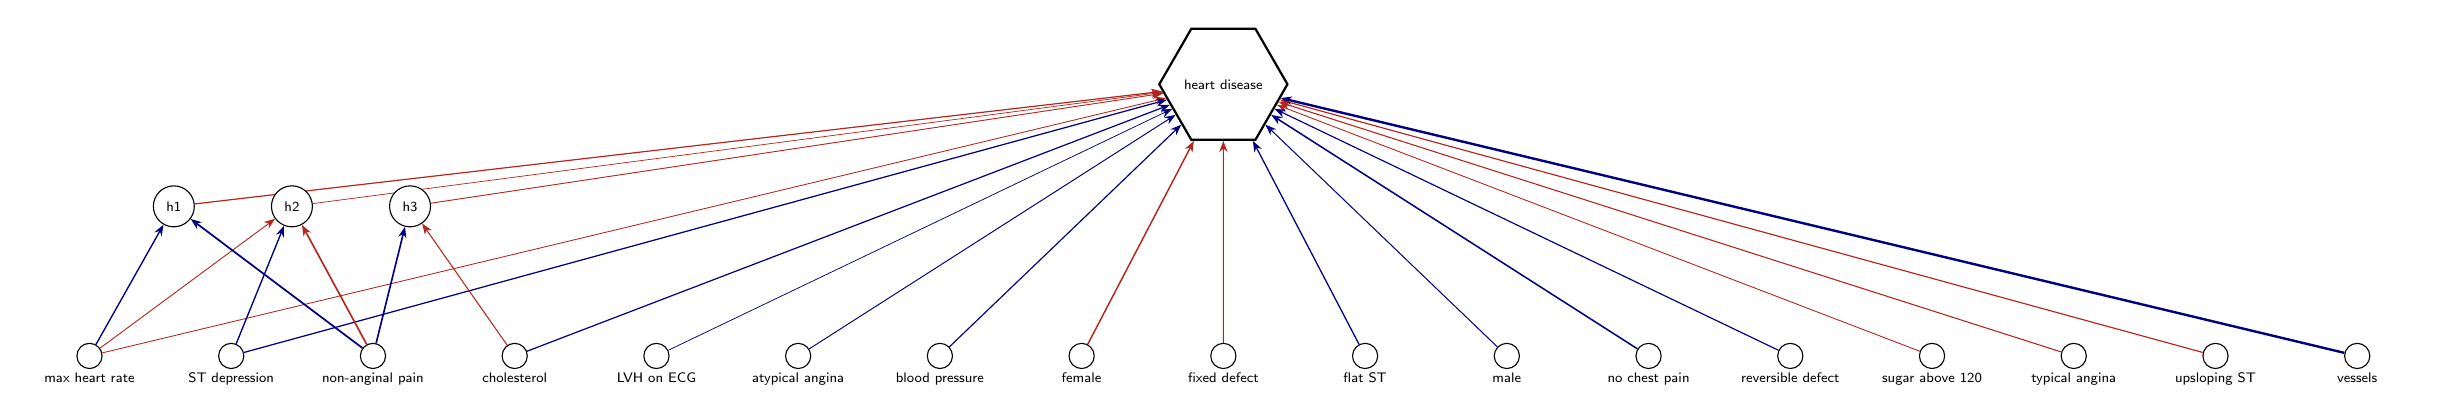
\begin{tikzpicture}[
  font=\sffamily\scriptsize, >={Stealth[length=1.4mm]},
  inp/.style={draw, circle, fill=white, minimum size=3.2mm, inner sep=0pt},
  hid/.style={draw, circle, fill=white, minimum size=5.2mm, inner sep=0.5pt, font=\sffamily\tiny},
  exitbox/.style={draw, thick, rectangle, fill=white, align=center, text width=17mm, minimum height=5mm, inner sep=1.5pt, font=\sffamily\tiny},
  sumbox/.style={draw, thick, dashed, rectangle, fill=white, align=center, text width=17mm, minimum height=5mm, inner sep=1.5pt, font=\sffamily\tiny},
  outp/.style={draw, thick, regular polygon, regular polygon sides=6, fill=white, minimum size=10mm, inner sep=0pt, font=\sffamily\tiny, align=center},
  stub/.style={draw, dashed, rounded corners=2pt, fill=white, align=center, inner sep=2pt, font=\sffamily\tiny, text width=15mm},
  inlab/.style={font=\sffamily\tiny, align=center, text width=15mm, inner sep=1pt, fill=white, fill opacity=0.8, text opacity=1},
  wpos/.style={draw=NavyBlue}, wneg/.style={draw=BrickRed}, wagg/.style={draw=black!45, line width=1.2pt},
  wmix/.style={draw=Plum},
]
\node[inp] (ninxxfbsx1) at (23.4,0.0) {};
\path (ninxxfbsx1.south) node[inlab, anchor=north] (labninxxfbsx1) {sugar above 120};
\node[inp] (ninxxrestecgx2) at (7.2,0.0) {};
\path (ninxxrestecgx2.south) node[inlab, anchor=north] (labninxxrestecgx2) {LVH on ECG};
\node[inp] (ninxxthalach) at (0.0,0.0) {};
\path (ninxxthalach.south) node[inlab, anchor=north] (labninxxthalach) {max heart rate};
\node[inp] (ninxxoldpeak) at (1.8,0.0) {};
\path (ninxxoldpeak.south) node[inlab, anchor=north] (labninxxoldpeak) {ST depression};
\node[inp] (ninxxslopex1) at (27.0,0.0) {};
\path (ninxxslopex1.south) node[inlab, anchor=north] (labninxxslopex1) {upsloping ST};
\node[inp] (ninxxsexx0) at (12.6,0.0) {};
\path (ninxxsexx0.south) node[inlab, anchor=north] (labninxxsexx0) {female};
\node[inp] (ninxxslopex2) at (16.2,0.0) {};
\path (ninxxslopex2.south) node[inlab, anchor=north] (labninxxslopex2) {flat ST};
\node[inp] (ninxxca) at (28.8,0.0) {};
\path (ninxxca.south) node[inlab, anchor=north] (labninxxca) {vessels};
\node[inp] (ninxxthalx6) at (14.4,0.0) {};
\path (ninxxthalx6.south) node[inlab, anchor=north] (labninxxthalx6) {fixed defect};
\node[inp] (ninxxthalx7) at (21.6,0.0) {};
\path (ninxxthalx7.south) node[inlab, anchor=north] (labninxxthalx7) {reversible defect};
\node[inp] (ninxxsexx1) at (18.0,0.0) {};
\path (ninxxsexx1.south) node[inlab, anchor=north] (labninxxsexx1) {male};
\node[inp] (ninxxcpx1) at (25.2,0.0) {};
\path (ninxxcpx1.south) node[inlab, anchor=north] (labninxxcpx1) {typical angina};
\node[inp] (ninxxcpx2) at (9.0,0.0) {};
\path (ninxxcpx2.south) node[inlab, anchor=north] (labninxxcpx2) {atypical angina};
\node[inp] (ninxxcpx3) at (3.6,0.0) {};
\path (ninxxcpx3.south) node[inlab, anchor=north] (labninxxcpx3) {non-anginal pain};
\node[inp] (ninxxcpx4) at (19.8,0.0) {};
\path (ninxxcpx4.south) node[inlab, anchor=north] (labninxxcpx4) {no chest pain};
\node[inp] (ninxxtrestbps) at (10.8,0.0) {};
\path (ninxxtrestbps.south) node[inlab, anchor=north] (labninxxtrestbps) {blood pressure};
\node[inp] (ninxxchol) at (5.4,0.0) {};
\path (ninxxchol.south) node[inlab, anchor=north] (labninxxchol) {cholesterol};
\node[outp] (n0) at (14.4,3.45) {heart disease};
\node[hid] (n2472) at (1.071,1.9) {h1};
\node[hid] (n2596) at (2.571,1.9) {h2};
\node[hid] (n2863) at (4.071,1.9) {h3};
\begin{scope}[on background layer]
\draw[->, wneg, line width=0.32pt] (ninxxfbsx1) -- (n0);
\draw[->, wpos, line width=0.27pt] (ninxxrestecgx2) -- (n0);
\draw[->, wneg, line width=0.31pt] (ninxxthalach) -- (n0);
\draw[->, wpos, line width=0.49pt] (ninxxthalach) -- (n2472);
\draw[->, wneg, line width=0.33pt] (ninxxthalach) -- (n2596);
\draw[->, wpos, line width=0.45pt] (ninxxoldpeak) -- (n0);
\draw[->, wpos, line width=0.49pt] (ninxxoldpeak) -- (n2596);
\draw[->, wneg, line width=0.42pt] (ninxxslopex1) -- (n0);
\draw[->, wneg, line width=0.52pt] (ninxxsexx0) -- (n0);
\draw[->, wpos, line width=0.46pt] (ninxxslopex2) -- (n0);
\draw[->, wpos, line width=0.87pt] (ninxxca) -- (n0);
\draw[->, wneg, line width=0.35pt] (ninxxthalx6) -- (n0);
\draw[->, wpos, line width=0.42pt] (ninxxthalx7) -- (n0);
\draw[->, wpos, line width=0.37pt] (ninxxsexx1) -- (n0);
\draw[->, wneg, line width=0.39pt] (ninxxcpx1) -- (n0);
\draw[->, wpos, line width=0.35pt] (ninxxcpx2) -- (n0);
\draw[->, wpos, line width=0.63pt] (ninxxcpx3) -- (n2472);
\draw[->, wneg, line width=0.59pt] (ninxxcpx3) -- (n2596);
\draw[->, wpos, line width=0.59pt] (ninxxcpx3) -- (n2863);
\draw[->, wpos, line width=0.55pt] (ninxxcpx4) -- (n0);
\draw[->, wpos, line width=0.42pt] (ninxxtrestbps) -- (n0);
\draw[->, wpos, line width=0.44pt] (ninxxchol) -- (n0);
\draw[->, wneg, line width=0.38pt] (ninxxchol) -- (n2863);
\draw[->, wneg, line width=0.43pt] (n2472) -- (n0);
\draw[->, wneg, line width=0.26pt] (n2596) -- (n0);
\draw[->, wneg, line width=0.33pt] (n2863) -- (n0);
\end{scope}
\end{tikzpicture}}%
\caption{The network as trained, before any explanation, in full. Blue: positive weight (raises the score); red: negative weight (lowers it); thicker: larger weight. Orange outline and up arrow: raises the final prediction; teal and down arrow: lowers it; grey and double arrow: depends. Not used (no connection): age, sugar 120 or less, normal ECG, ST-T abnormal ECG, no exercise pain, exercise pain, downsloping ST, normal thallium, thallium code 4.}
\label{fig:hearts2c3:raw}
\end{figure}
\end{landscape}
\end{drafted}
\clearpage
\end{document}
